\documentclass[12pt,a4paper]{article}
\usepackage{graphicx}
\usepackage{csquotes}
\usepackage{centernot}
\usepackage{mathtools}
\usepackage{amsfonts}
\usepackage{algorithm}
\usepackage[title]{appendix}
\usepackage{amsthm}
\usepackage{caption}
\usepackage{array}
\usepackage{dsfont}
\usepackage{ amssymb }
\usepackage{blindtext}
\usepackage{hyperref}
\usepackage{amsmath}
\usepackage{breqn}
\usepackage{tikz}
\usepackage{pgfplots}
\renewcommand{\arraystretch}{1.3}
\usepackage[a4paper]{geometry}
\usepackage{multirow}
\usepackage{graphicx}
\usepackage[all]{xy}
\newtheorem{theorem}{Theorem}
\theoremstyle{definition}
\newtheorem{definition}{Definition}[section]
\theoremstyle{remark}
\newtheorem*{remark}{Remark}
\usepackage[noend]{algpseudocode}
\pgfmathdeclarefunction{poiss}{1}{%
	\pgfmathparse{(#1^x)*exp(-#1)/(x!)}%
}

\algrenewcommand\algorithmicrequire{\textbf{Input:}}
\newcommand\ddfrac[2]{\frac{\displaystyle #1}{\displaystyle #2}}
\newcommand\at[2]{\left.#1\right|_{#2}}
\usepackage{mathtools}
\DeclarePairedDelimiter{\ceil}{\lceil}{\rceil}
\graphicspath{ {images} }
%opening
\title{Bayesian Regression with COVID-19 spread data}
\author{Michele Guerrini, Davide Mozzi, Carlos Santillán}
\begin{document}
	\maketitle
	\begin{abstract}
		We present a Bayesian regression model for predicting the number of patients in a hospital and in its ICU with COVID-19, given the number of patients in the same hospital and in the ICU, the number of new positive subjects and the region color of the previous week.
	\end{abstract}
	
	\tableofcontents
	\newpage
	\section{Problem Description and Dataset}
	\subsection{Problem description}
	We are given the problem of predicting the number of patients in a hospital and the ICU 7 days from the current date. The prediction is based on the current date's patients both in the hospital and the ICU, new positive subjects, the average number of new positive subjects over the previous 7 days, and the color of the region. We tackle the problem via Bayesian regression.
	\subsection{Dataset description}
	The dataset contains 205 entries. Each entry corresponds to a date with the following covariates:
	\begin{enumerate}
		\item \textbf{newpos:} Number of newly detected COVID-19 positive subjects. An integer value.
		\item \textbf{intcar:} 	Number of COVID patients in the ICU. An integer value.
		\item \textbf{hosp:} Number of COVID patients at the hospital. An integer value.
		\item \textbf{newpos\_av7D:} Average number of newly detected COVID-19 positive subjects over the previous 7 days. A float value.
		\item \textbf{color:} Color of the region over the previous 7 days. String that can contain the following values: \textit{Bianca}, \textit{Gialla}, \textit{Arancione}, \textit{Rossa}.
		\item \textbf{day:} Current date. String in R date format.
		\item \textbf{hospH8:} A target variable, the number of COVID patients at the hospital 7 days from now.
		\item \textbf{intcarH8:} A target variable, the number of COVID patients in the ICU 7 days from now.
		\item \textbf{dayH8:} The current date plus 7 days. 
	\end{enumerate}
	We will extend this by adding a categorical variable \textbf{season}, which will have values: \textit{winter}, \textit{spring}, \textit{summer}, \textit{fall}.

 
	\subsection{Data exploration}
	We start by looking at a pairs plot of the \textbf{newpos}, \textbf{intcar}, \textbf{hosp}, \textbf{newpos-avg7D}, and \textbf{hospH8}. The pairs plot contains a kernel density estimation of the distribution along the diagonal, the estimations are distinguished by color of the region. We also see the scatter plots for each pair of covariates and the correlations between them for each region.
	\begin{figure}[htb!]
		\centering
		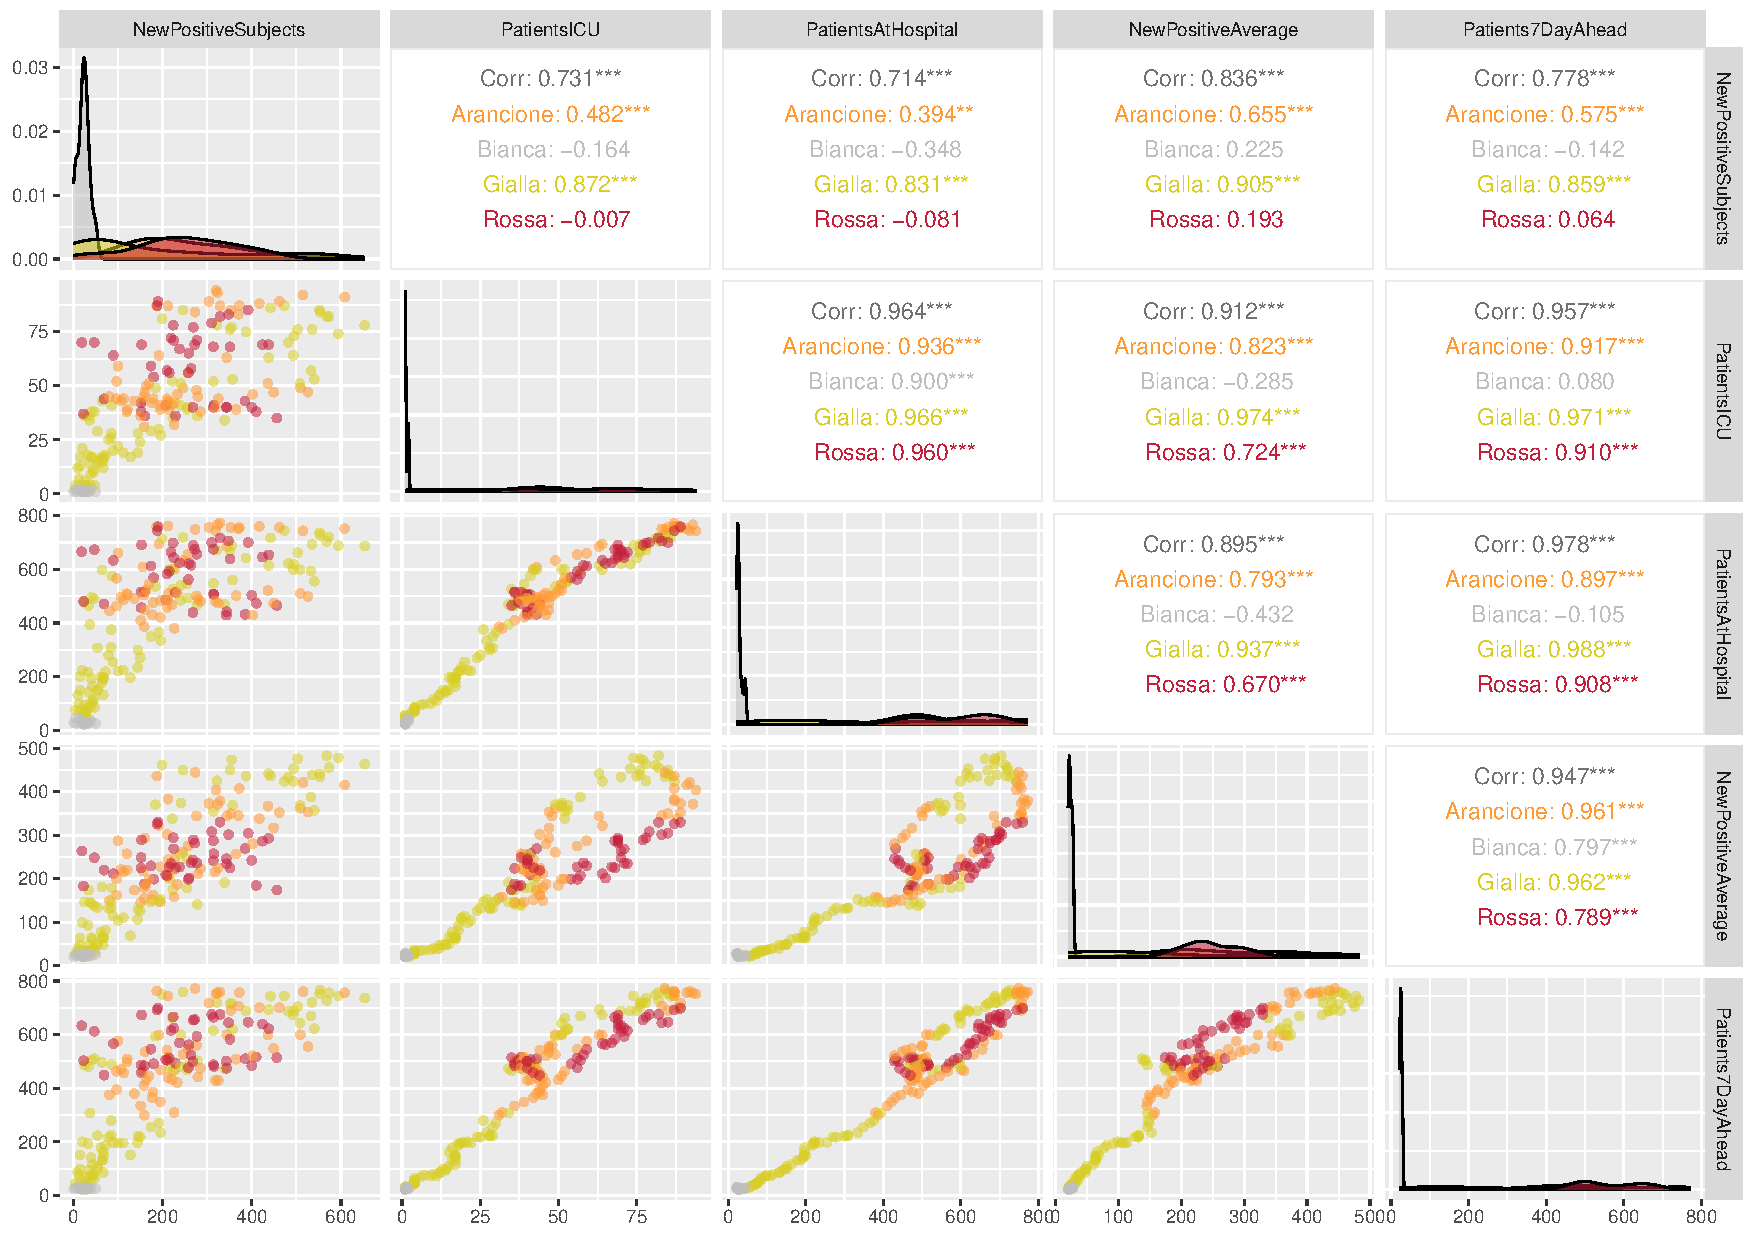
\includegraphics[width=150mm, height=115mm,scale=0.5]{corrplot.pdf}
			\caption{Pairs plot between the covariates and the number of patients at the hospital 7 days from now}
	\end{figure}
	
	We can immediately see an almost linear relationship between the number of patients in the ICU and those at the hospital, suggesting that we may remove one of them. The density plots are as we would expect, the white regions (lower COVID-19 presence) have all the mass concentrated around low values of the features, while the other regions are more spread out and have a center of mass further to the right (higher values). We also see that the relationship between the number of patients at the hospital, and that of 7 days in the future could be linear.
	
	\newpage
	We now look at the correlations with the number of patients in the ICU
		\begin{figure}[htb!]
		\centering
		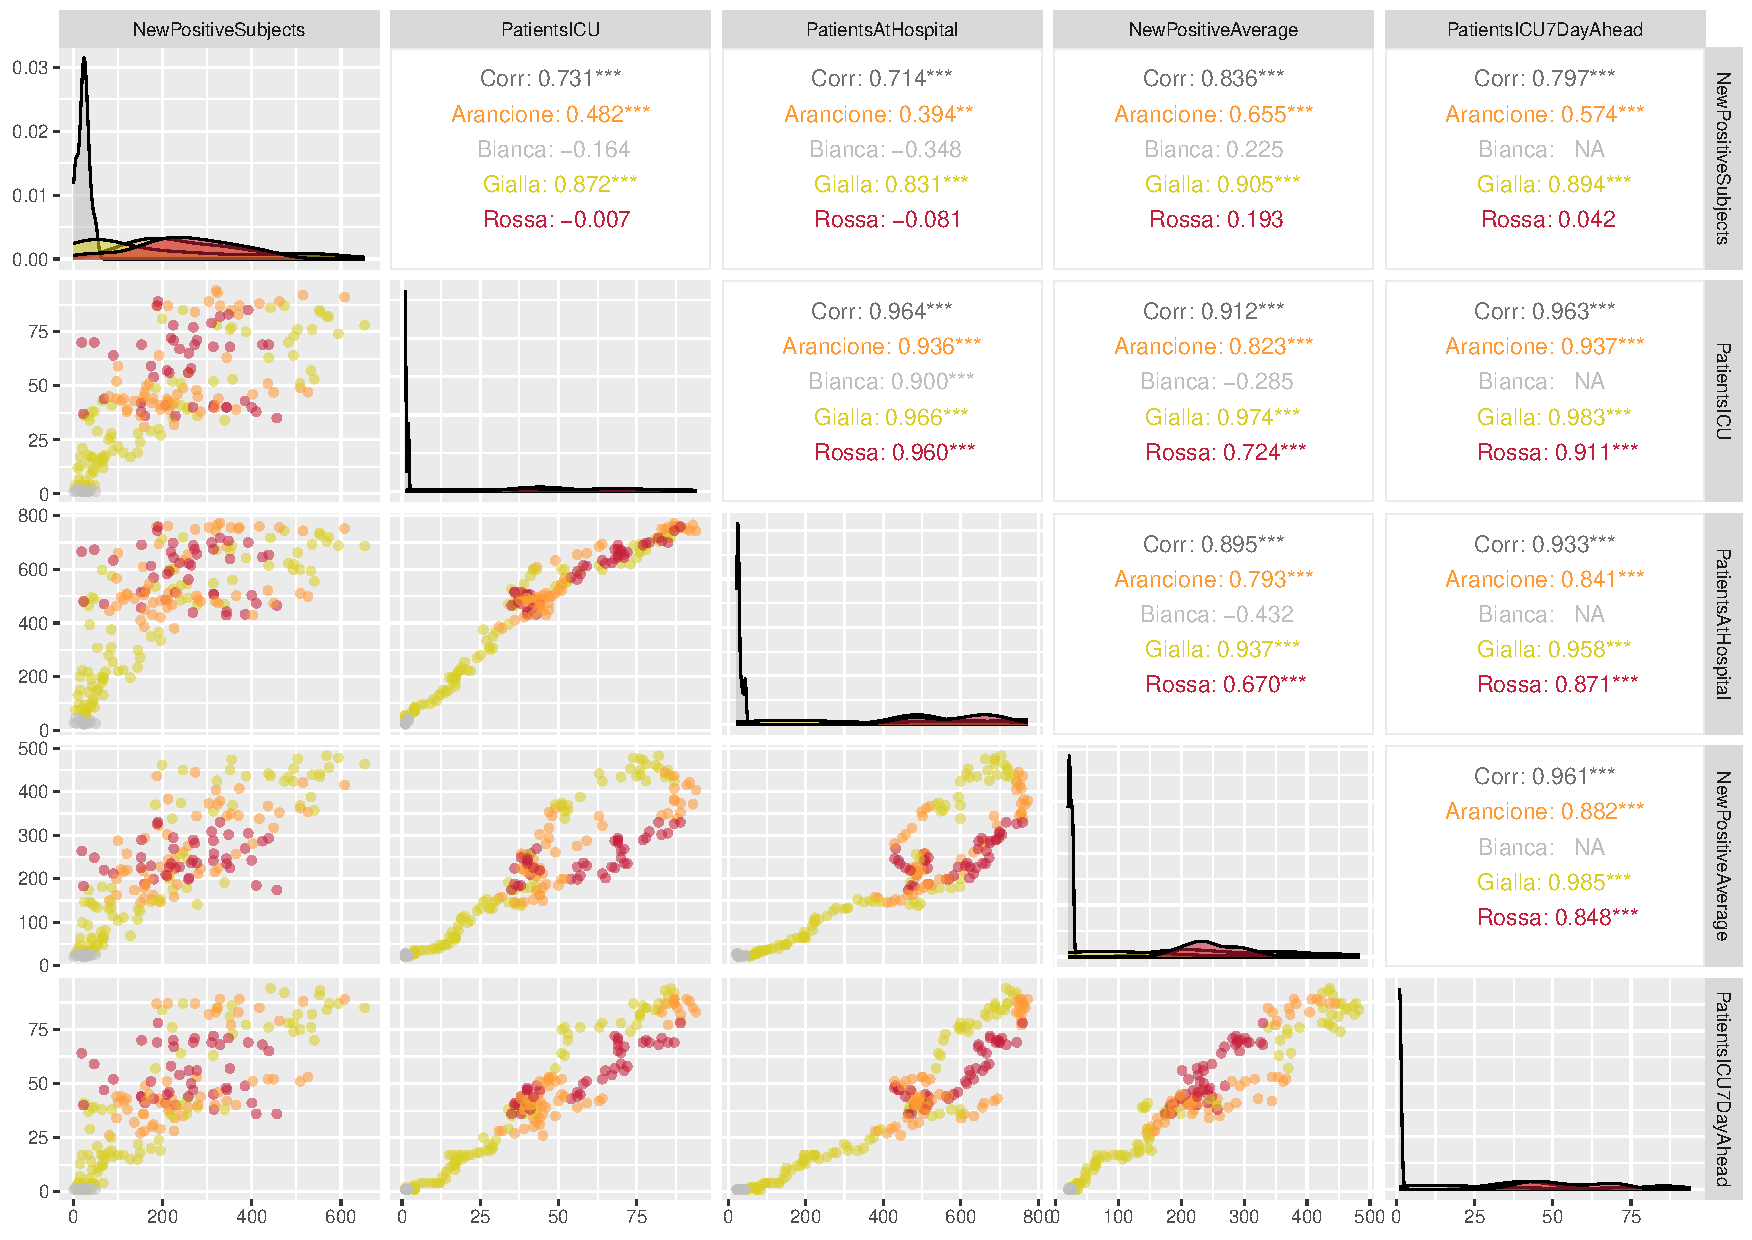
\includegraphics[width=150mm, height=115mm,scale=0.5]{corrplot1.pdf}
		\caption{Pairs plot between the covariates and the number of patients in the ICU 7 days from now}
	\end{figure}
	
	
	Again, for some of the covariates, the relationship appears to be linear w.r.t. the target variable. Note that where the correlation is marked NA the value is zero. We used the Pearson correlation coefficient $r_{X,Y}$, defined as
	\begin{align*}
		r_{X,Y} = \frac{\sum(x_i-\overline{x})(y_i-\overline{y})}{\sqrt{\sum(x_i-\overline{x})^2\sum(y_i-\overline{y})^2}}
	\end{align*}


    Now we qualitatively assess how much each covariate varies via boxplots (Figure 3). A boxplot allows us to see the spread of our data, the boxes themselves contain the interquantile range, the whiskers show the range of the rest of the data. We also mean center the covariates.
    	\begin{figure}[htb!]
    	\centering
    	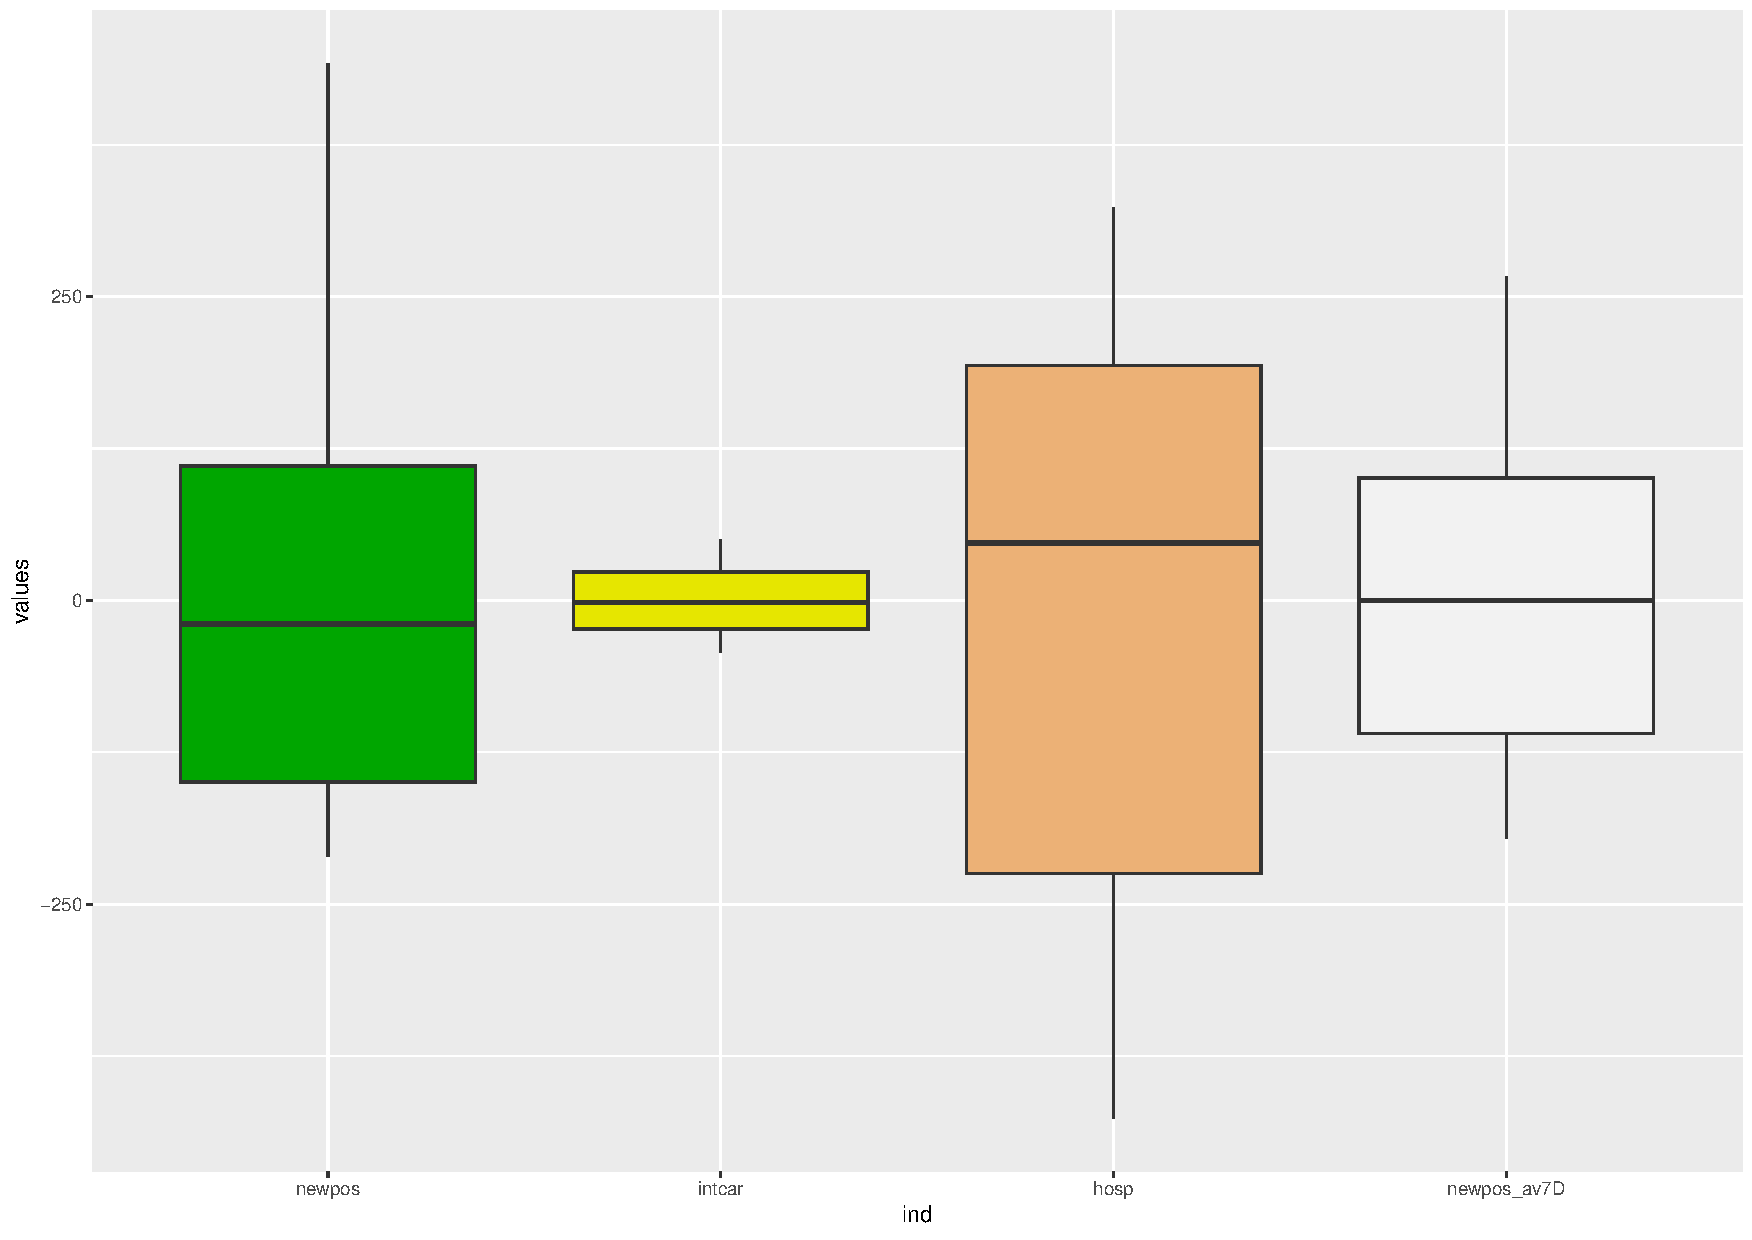
\includegraphics[width=100mm, height=80mm,scale=0.5]{box.pdf}
    	\caption{Boxplot of the mean-centered covariates}
    \end{figure}
    
    Since some of the covariates vary greatly w.r.t. to others, see \textbf{intcar} and \textbf{hosp}, it could be a convenient to normalize them. 

Lastly, we take a look at the correlation matrices of the covariates. Figure 4 shows the full correlation matrix, no distinction made between regions. 

Figure 5 shows the correlation matrix for each region.
    
\begin{figure}[htb!]
	\centering
	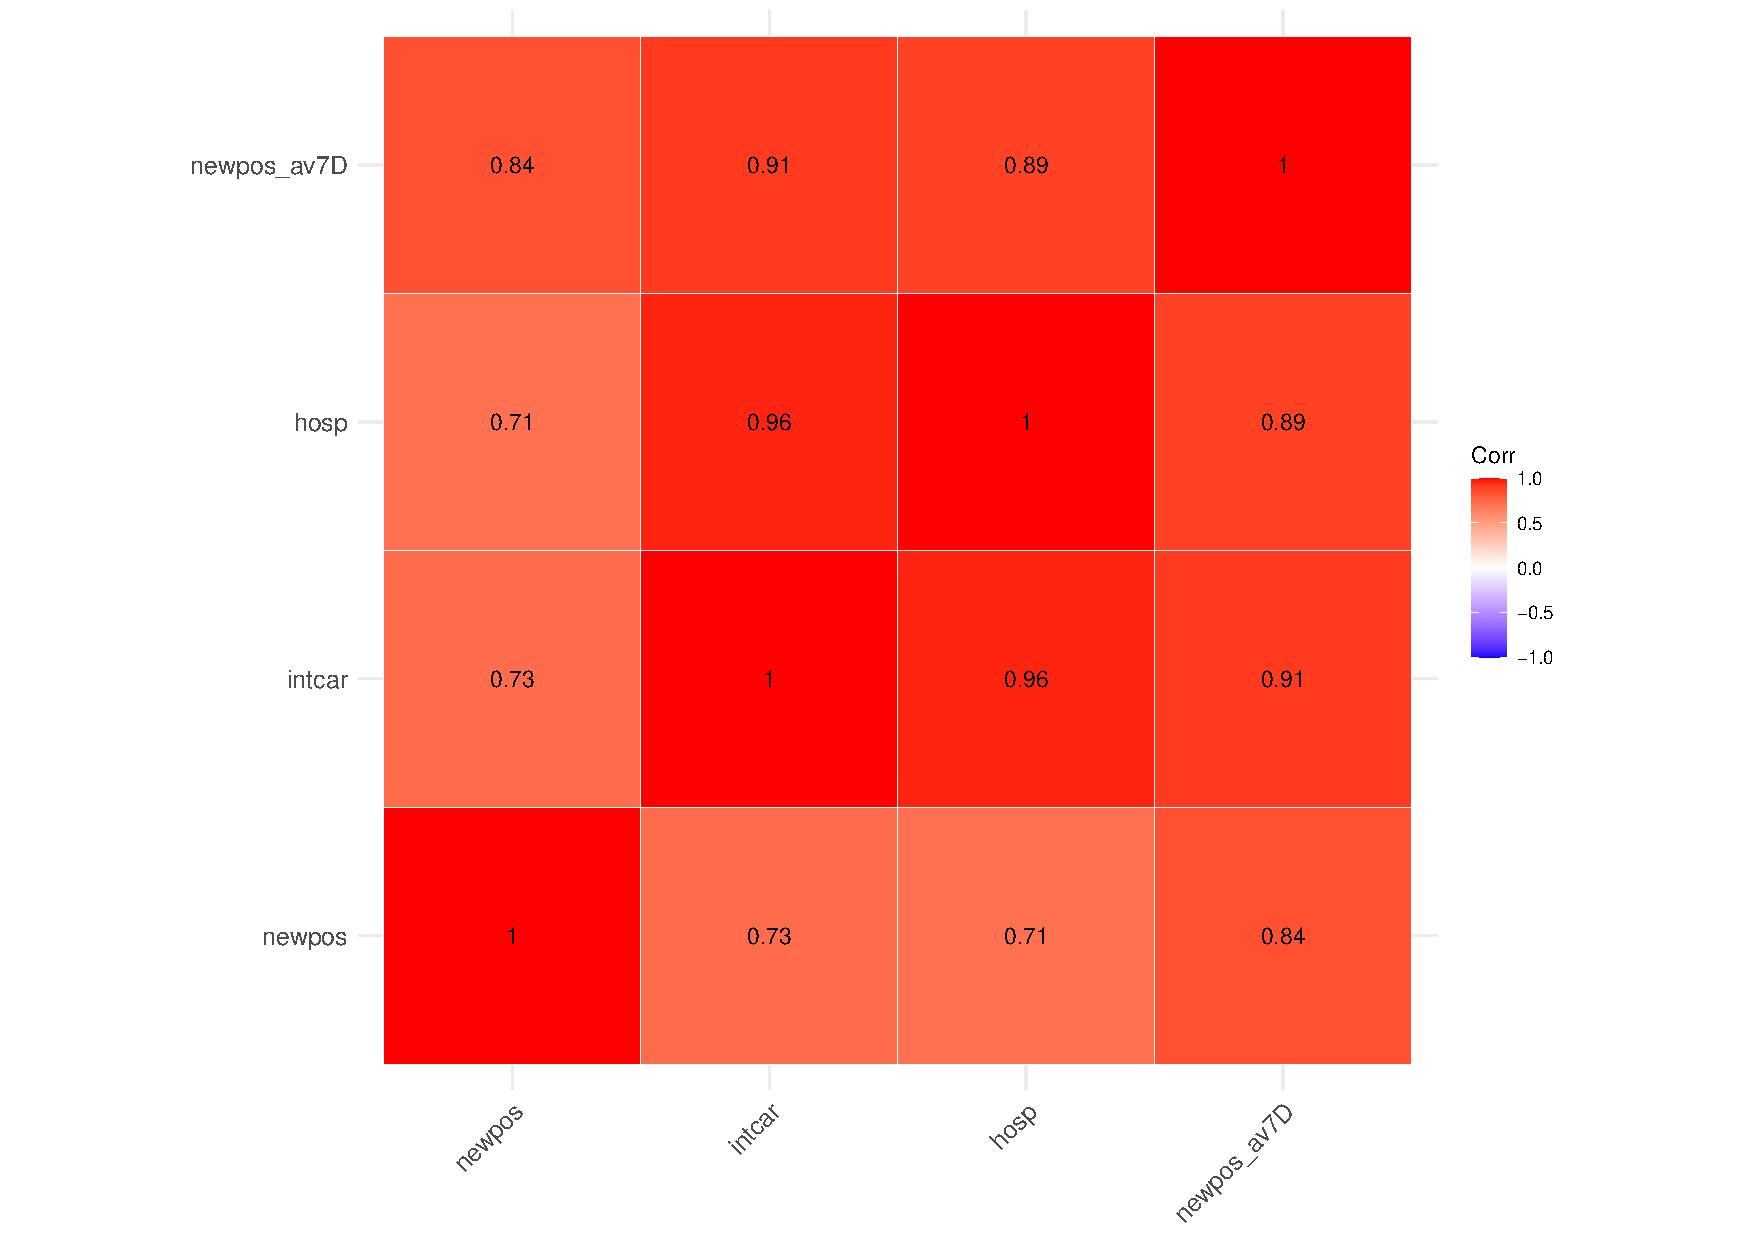
\includegraphics[width=75mm, height=60mm,scale=0.5]{corrmatrix.pdf}
	\caption{Correlation matrix of the covariates}
\end{figure}
\begin{figure}[htb!]
	\centering
	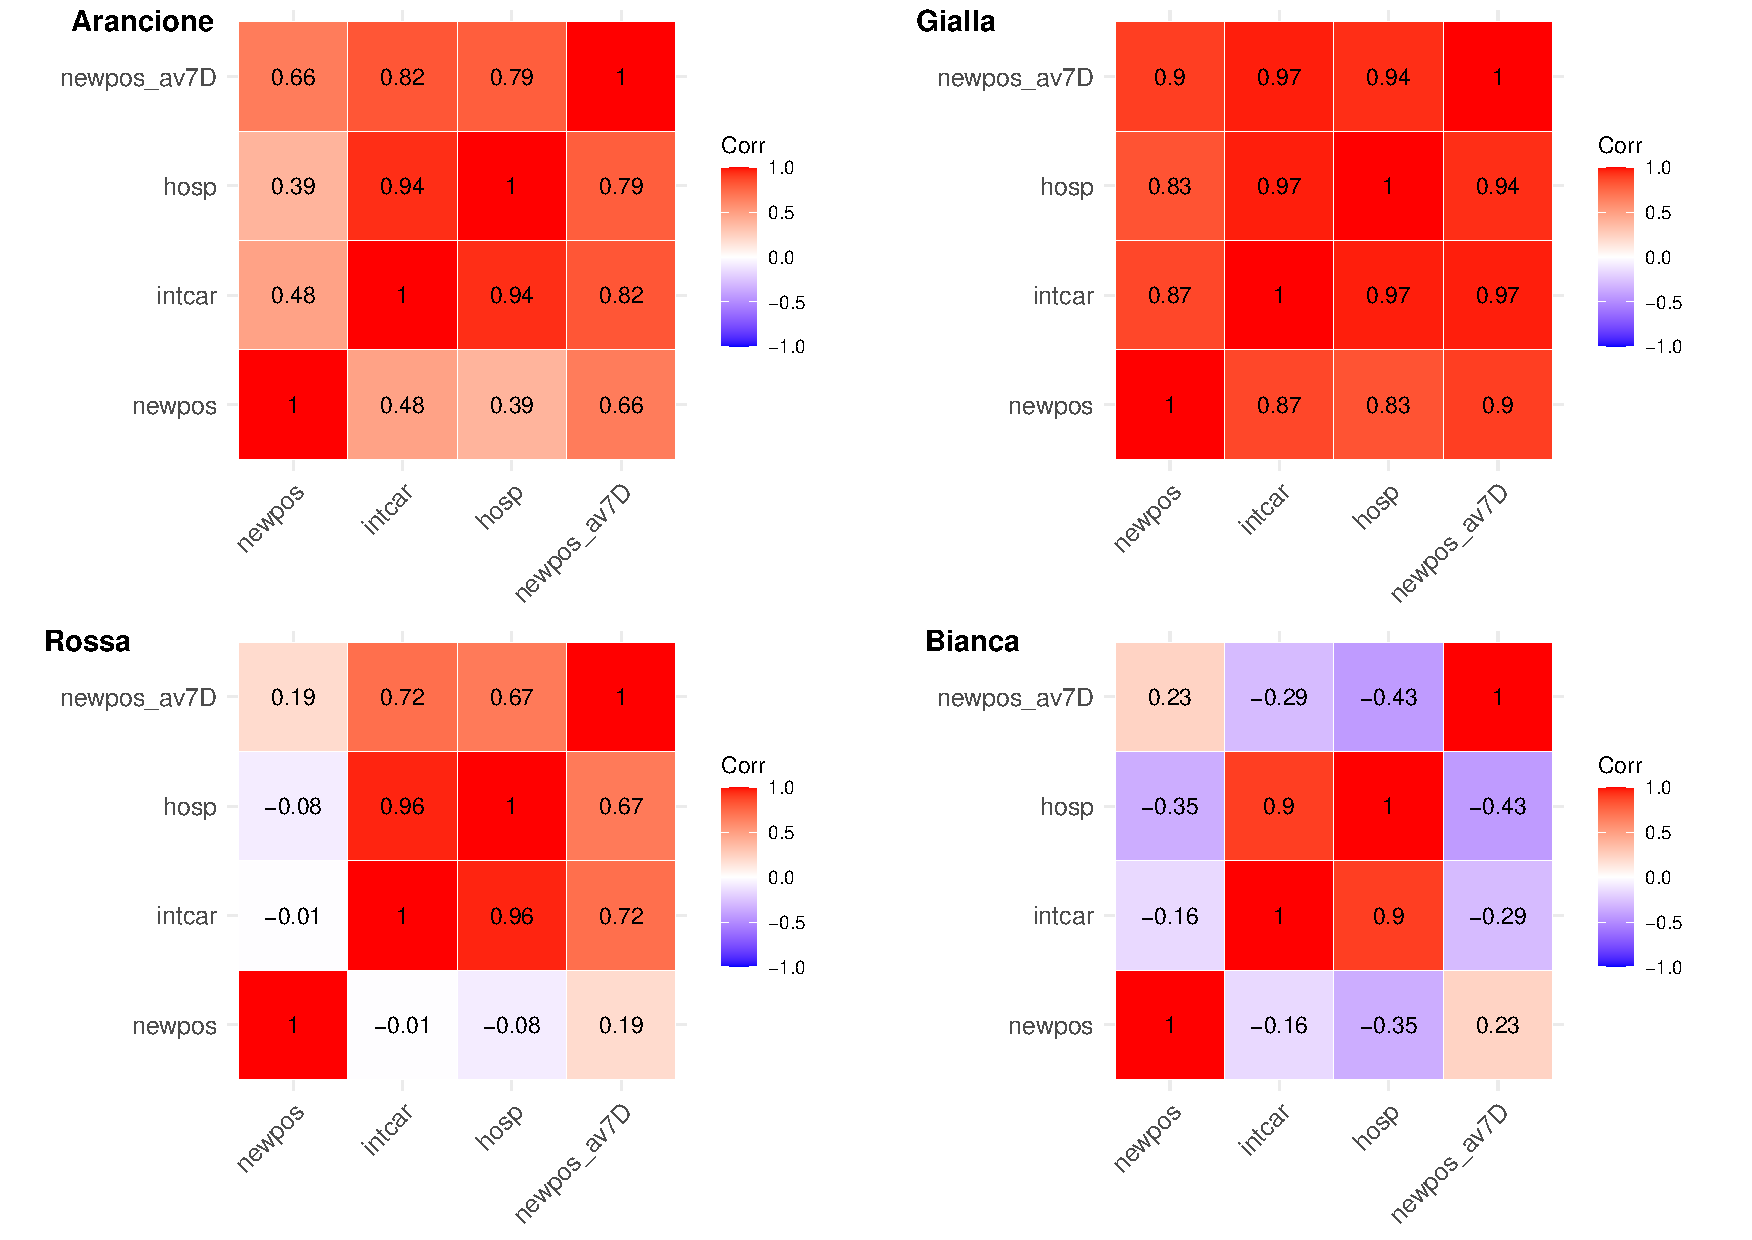
\includegraphics[width=130mm, height=100mm,scale=0.5]{corrmat2.pdf}
	\caption{Correlation matrix of the covariates per color of the region}
\end{figure}


Before proceeding, we shuffle the dataset and normalize the covariates, but not the target variables.

\clearpage




\section{Model specification}
\subsection{Likelihood and prior}
In the Bayesian setting, we use a Gaussian likelihood
\begin{align*}
	y|\beta,\sigma^2,X \sim \mathcal{N}_n(X\beta,\sigma^2I_n)
\end{align*}

For the prior we initially use default one provided by BAS, an approximation of the Zellner-Siow prior, with the hyperparameter $\alpha$ set to 1. This prior is defined as:
	\begin{align*}
	\beta = (\beta_1, \dots, \beta_k)|\sigma^2, \alpha, X &\sim \mathcal{N}_k(0, \alpha\sigma^2(X^TX)^{-1}) \\
	\sigma^2|X,\alpha &\sim \pi(\sigma^2) = \sigma^{-2} \\
	1/\alpha &\sim \pi_0 = \Gamma(1/2, n/2)
\end{align*}

We try to predict each target separately and start with \textbf{hospH8}, we consider a model with all the covariates. In particular, \textbf{color} is considered a categorical variable, which was transformed into 3 binary covariates via one-hot encoding. The model is
\begin{dmath*}
	\textbf{hospH8} = \beta_0 + \beta_1\textbf{gialla} + \beta_2\textbf{arancione} + \beta_3\textbf{rossa} + \beta_4\textbf{newpos} + \beta_5\textbf{intcar} + \beta_6\textbf{hosp} + \beta_7\textbf{newpos\_av7D} +  \varepsilon
\end{dmath*}

Since we are only using one model which always includes these covariates the probability of them belonging to the model is always 1.  Table 1 shows the posterior means and standard deviations of the coefficients\footnote{Do not confuse them with the actual covariates, these refer to the coefficents $\beta_i$ of $i$-th covariate}

We perform inference on the test set, for which BAS uses the posterior predictive distribution. We recall that in general the predictive posterior distribution is computed as 
	\begin{align*}
	\int \pi(y_{\text{new}}|\sigma^2,\beta,X_{\text{new}})\pi(\sigma^2,\beta|y,X)\,d\sigma^2d\beta
\end{align*}

To evaluate the results we use k-fold cross-validation, computing and averaging the mean square error (MSE):
\begin{align*}
	\text{MSE} = \frac{1}{n}\sum_{i=1}^{n}(y_i-\hat{y_i})^2
\end{align*}
where $y_i$ is the actual number of people hospitalized after 7 days, and $\hat{y_i}$ is our prediction. We obtain a MSE of 938.4436.

For the target variable \textbf{intcarH8} we consider the same model

\begin{dmath*}
	\textbf{intcarH8} = \beta_0 + \beta_1\textbf{gialla} + \beta_2\textbf{arancione} + \beta_3\textbf{rossa} + \beta_4\textbf{newpos} + \beta_5\textbf{intcar} + \beta_6\textbf{hosp} + \beta_7\textbf{newpos\_av7D} + \varepsilon
\end{dmath*}

The MSE is 23.4831. We show a more in-depth posterior analysis with the final model. Please note that the covariates in the test set are normalized with the training set's mean and standard deviation. 

\subsubsection*{Zellner's g-prior}

We change prior to Zellner's g-prior, of the form
    \begin{align*}
    \beta = (\beta_1,\dots, \beta_k)|\sigma^2 &\sim \mathcal{N}_k(0, \alpha\sigma^2(X^TX)^{-1}) \\
    (\beta_0, \sigma^2) &\sim \pi(\beta_0, \sigma^2) = \sigma^{-2}
    \end{align*}
For the hyperparameter we chose a value of $\alpha = 100$ and obtain an MSE of 943.1065 for the target \textbf{hospH8} and of 23.55807 for \textbf{intcarH8}.

\subsection{Model selection}
To perform model selection we use the \textbf{Bayesian information criterion (BIC)} defined as
    \begin{align*}
    BIC = -2\ln\left[\mathcal{L}\left(\mathbf{y} \mid \hat{\beta},\, \hat{\sigma}^2,\, M\right)\right]+(p+1)\ln(n)
    \end{align*}
This approach uses a non-informative prior to train a large number of models trying different subsets of covariates and then chooses the best one based on the above criterion, which is the one with lowest BIC.\\

In Table 1 we show the posterior probabilities that each covariate is contained in the model for the prediction of \textbf{hospH8}. In Table 2 we see the same for \textbf{intcarH8}.
\begin{table}[!htb]
	\centering
	\begin{tabular}{|c|c|}
		\hline
		Coefficient          & Posterior \\ \hline
		Intercept          & 1.0000000                   \\ \hline
		\textbf{gialla}    & 0.1736033                  \\ \hline
		\textbf{arancione} & 0.1845924                   \\ \hline
		\textbf{rossa}     & 0.9420397                     \\ \hline
		\textbf{newpos}    & 0.1676675                  \\ \hline
		\textbf{intcar}    & 0.4934792                \\ \hline
		\textbf{hosp}      & 1.0000000        \\ \hline
			\textbf{newpos\_av7D}      & 1.0000000        \\ \hline
	\end{tabular}
	\caption{Probabilities of each covariate for \textbf{hospH8}}
\end{table}

\begin{table}[!htb]
	\centering
	\begin{tabular}{|c|c|}
		\hline
		Coefficient          & Posterior \\ \hline
		Intercept          & 1.0000000                   \\ \hline
		\textbf{gialla}    &0.09773376                 \\ \hline
		\textbf{arancione} & 0.99781126               \\ \hline
		\textbf{rossa}     &0.11141621                 \\ \hline
		\textbf{newpos}    &0.14062014             \\ \hline
		\textbf{intcar}    &1.0000000            \\ \hline
		\textbf{hosp}      &0.08919494       \\ \hline
		\textbf{newpos\_av7D}      & 1.0000000        \\ \hline
	\end{tabular}
	\caption{Probabilities of each covariate for \textbf{intcarH8}}
\end{table}

As we can see we certainly want to include the covariates \textbf{rossa}, \textbf{hosp}, and \textbf{newpos\_av7D} in our model for \textbf{hospH8} and \textbf{arancione}, \textbf{intcar}, and \textbf{newpos\_av7D} for \textbf{intcarH8}.

In the case of \textbf{hospH8} the top 5 models have the following posterior probabilities
Table 3 and Table 4 show the posterior probabilities of the top 5 models for each target variable.

\begin{table}[!htb]
	\centering
	\begin{tabular}{|c|c|c|c|c|c|}
		\hline
		Models                & Model 1 & Model 2   & Model 3    & Model 4   & Model 5    \\ \hline
		Posterior probability & 0.3664  & 0.2734 & 0.0496 & 0.0478 & 0.0385 \\ \hline
	\end{tabular}
	\caption{Posterior probabilities of the best 5 models for \textbf{hospH8}}
\end{table}

\begin{table}[!htb]
	\centering
	\begin{tabular}{|c|c|c|c|c|c|}
		\hline
		Models                & Model 1 & Model 2   & Model 3    & Model 4   & Model 5    \\ \hline
		Posterior probability & 0.6669  & 0.0877 & 0.0586 & 0.0514 & 0.0504 \\ \hline
	\end{tabular}
	\caption{Posterior probabilities of the best 5 models for \textbf{intcarH8}}
\end{table}

Figure 6 and Figure 7 show a heatmap-like plot of the posterior probabilities and the inclusion of covariates of each model.

\begin{figure}[!htb]
	\centering
	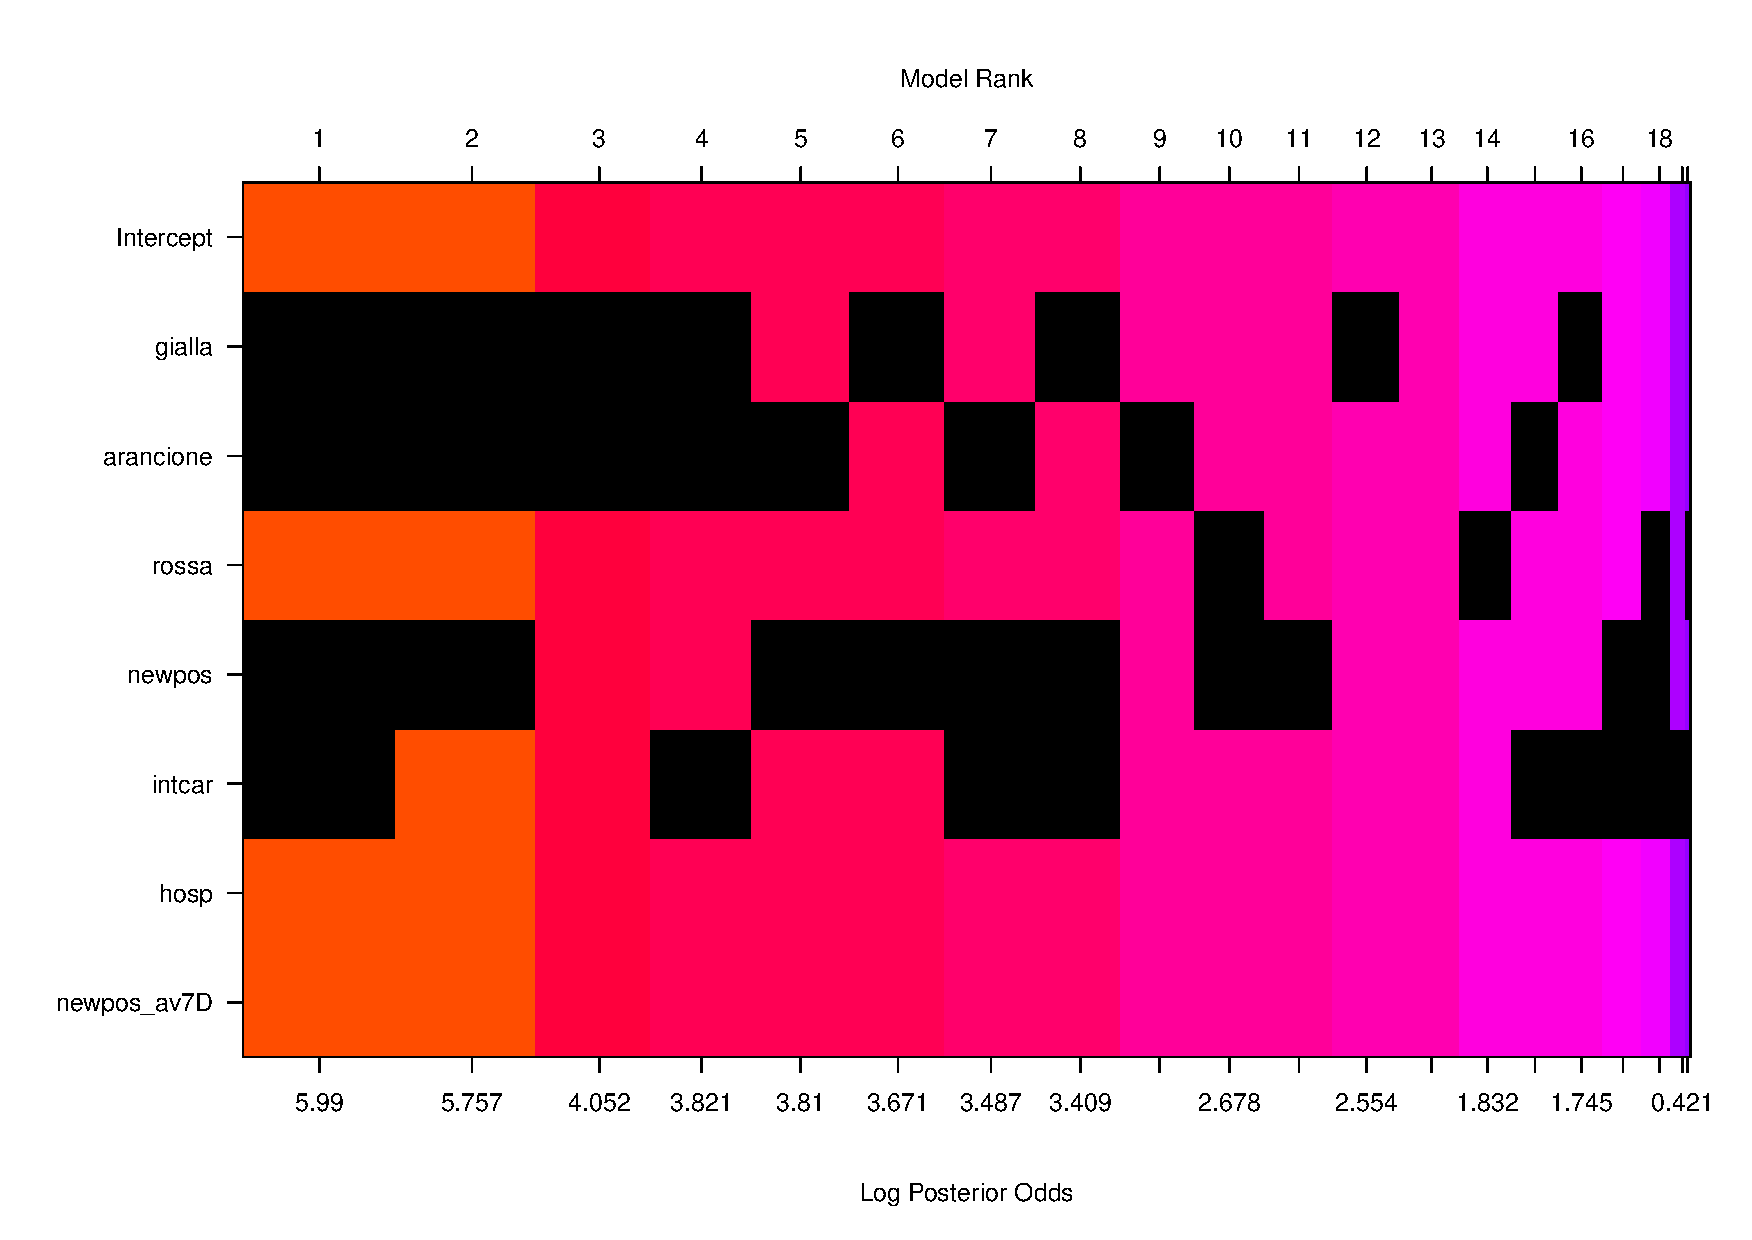
\includegraphics[width=100mm, height=60mm,scale=0.5]{modelranking.pdf}
	\caption{Model ranking and posterior probabilities }
\end{figure}

\begin{figure}[!htb]
	\centering
	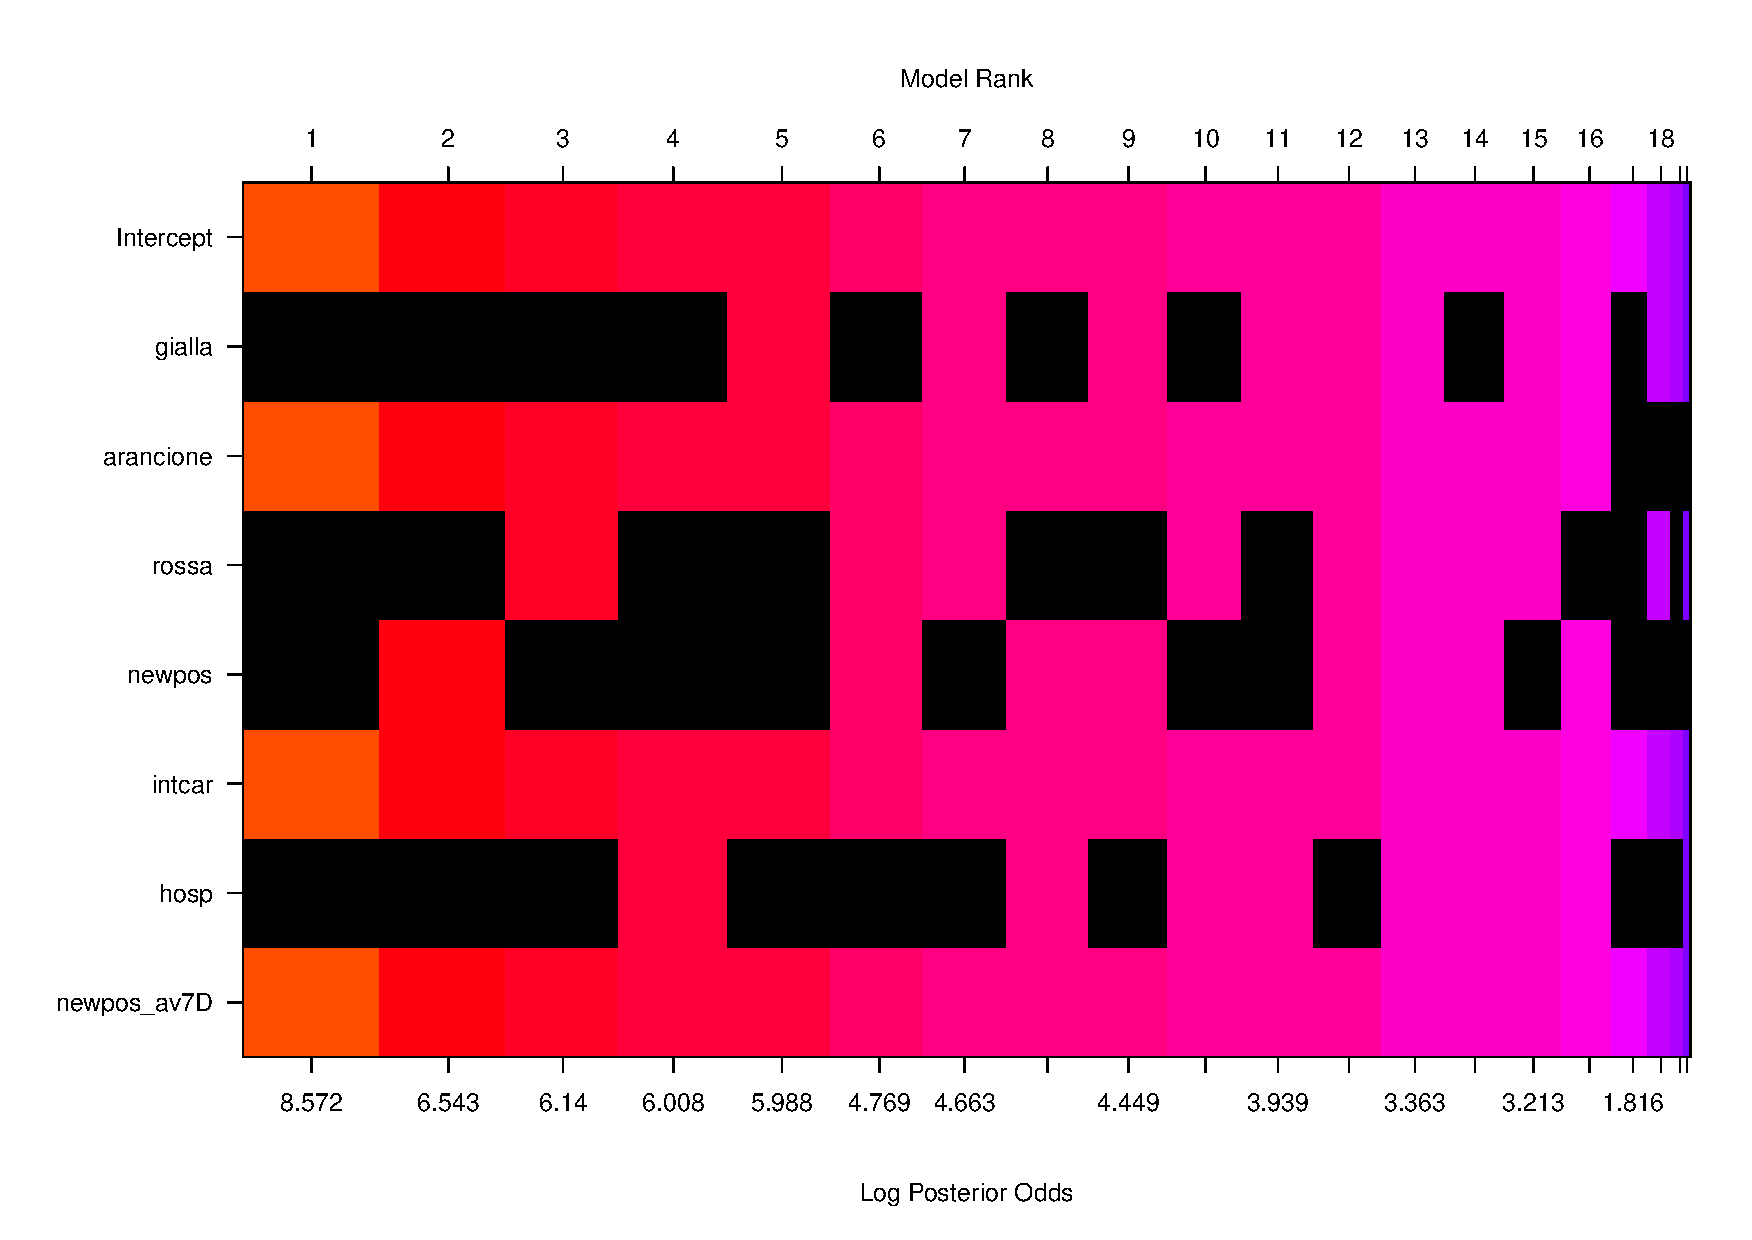
\includegraphics[width=100mm, height=60mm,scale=0.5]{ranking2.pdf}
	\caption{Model ranking for \textbf{intcarH8} }
\end{figure}

Since, for \textbf{hospH8}, none of the models have a posterior probability above 50\%, we do not choose the best model, Model 1, but we use Bayesian Model Averaging (BMA), the posterior probability of a quantity of interest $\Delta$, computed via BMA, is
\begin{align*}
	\pi(\Delta|\mathbf{y}) = \sum_{j=1}^{2^p}\pi(\Delta| M_j, \mathbf{y})\pi(M_j|\mathbf{y})
\end{align*}
where $p$ is the number of covariates.

We can therefore compute our predictions as a weighted average of each model's prediction, where the weights are the model's posterior probabilities
\begin{align*}
	\hat{Y} = \sum_{j=1}^{2^p}\hat{Y}^*_jp(M_j|X)
\end{align*}
The MSE for this aggregate model is 929.9491, sligthly better than the first model with all the covariates (while using only the Highest Probability Model the MSE is 950.7221).


For \textbf{intcarH8} the best model has a posterior probability of about 67\%, so we could try to use only that one to perform inference. So we choose the model
\begin{dmath*}
	\textbf{intcarH8} = \beta_0 + \beta_1\textbf{arancione} +  \beta_2\textbf{intcar} + \beta_3\textbf{newpos\_av7D} + \varepsilon
\end{dmath*}
which yields a MSE of 23.00852, slightly better than the one using all the covariates (while using BMA the MSE is 23.11804, which is very similar).

\newpage
\section{Posterior analysis}
\subsection{Posterior distributions }
We start with the aggregate model chosen for \textbf{hospH8}. The posterior distributions of the coefficients are
\begin{figure}[htb!]
	\centering
	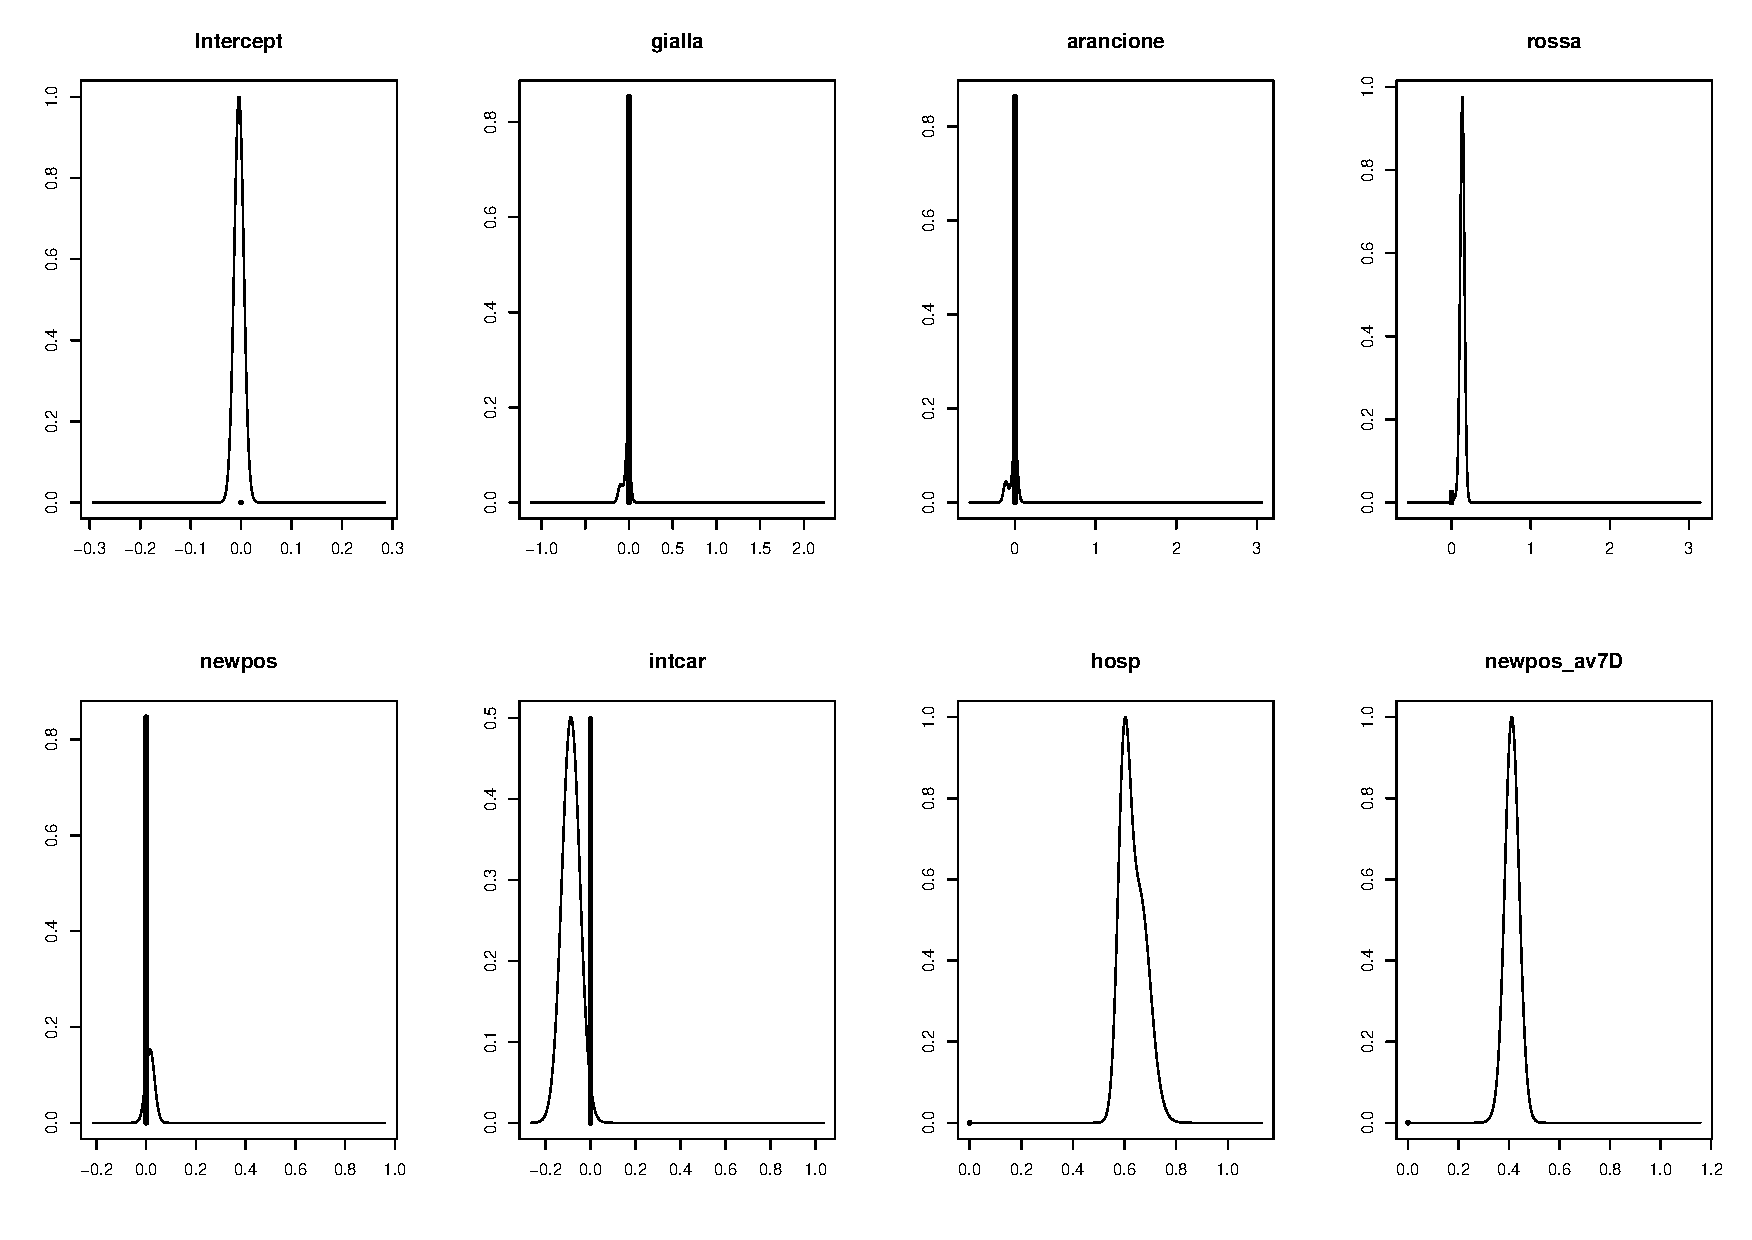
\includegraphics[width=155mm, height=90mm,scale=0.5]{posteriors_1.pdf}
	\caption{Posterior distributions of coefficients for best \textbf{hospH8} model}
\end{figure}

Judging by where they are centered we could say that the covariate \textbf{hosp} has more weight when performing inference w.r.t. \textbf{newpos\_av7D} and \textbf{rossa}.

In Figure 9 we show the credible intervals of the coefficients.
\begin{figure}[htb!]
	\centering
	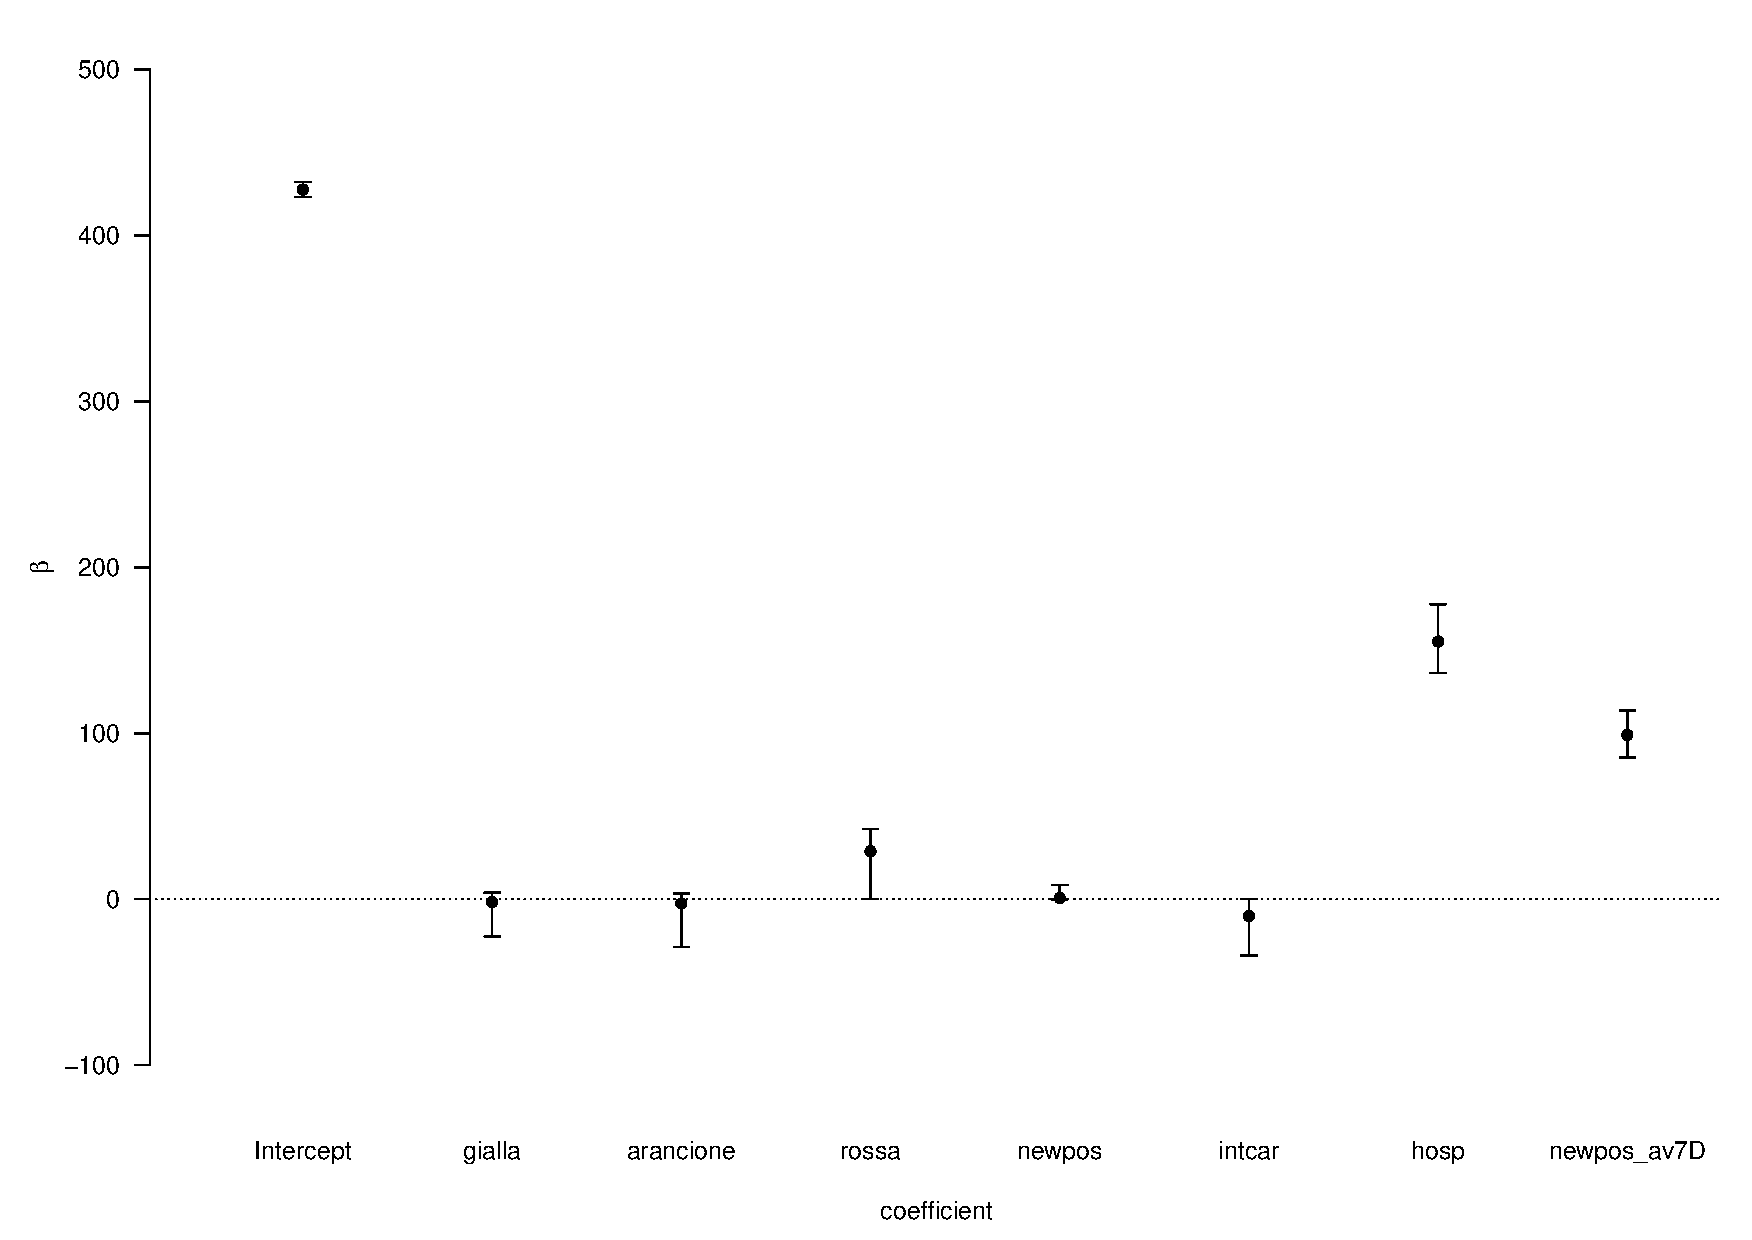
\includegraphics[width=155mm, height=90mm,scale=0.5]{crint1.pdf}
	\caption{95\% credible intervals for the coefficients in the \textbf{hospH8} model}
\end{figure}



We now consider the best model for predicting \textbf{intcarH8}. Figure 10 shows the posterior distribution of the coefficients. It appears that both \textbf{intcar} and \textbf{newpos\_av7D} have a higher weight w.r.t. \textbf{arancione}. Figure 11 shows the credible intervals.

\begin{figure}[htb!]
	\centering
	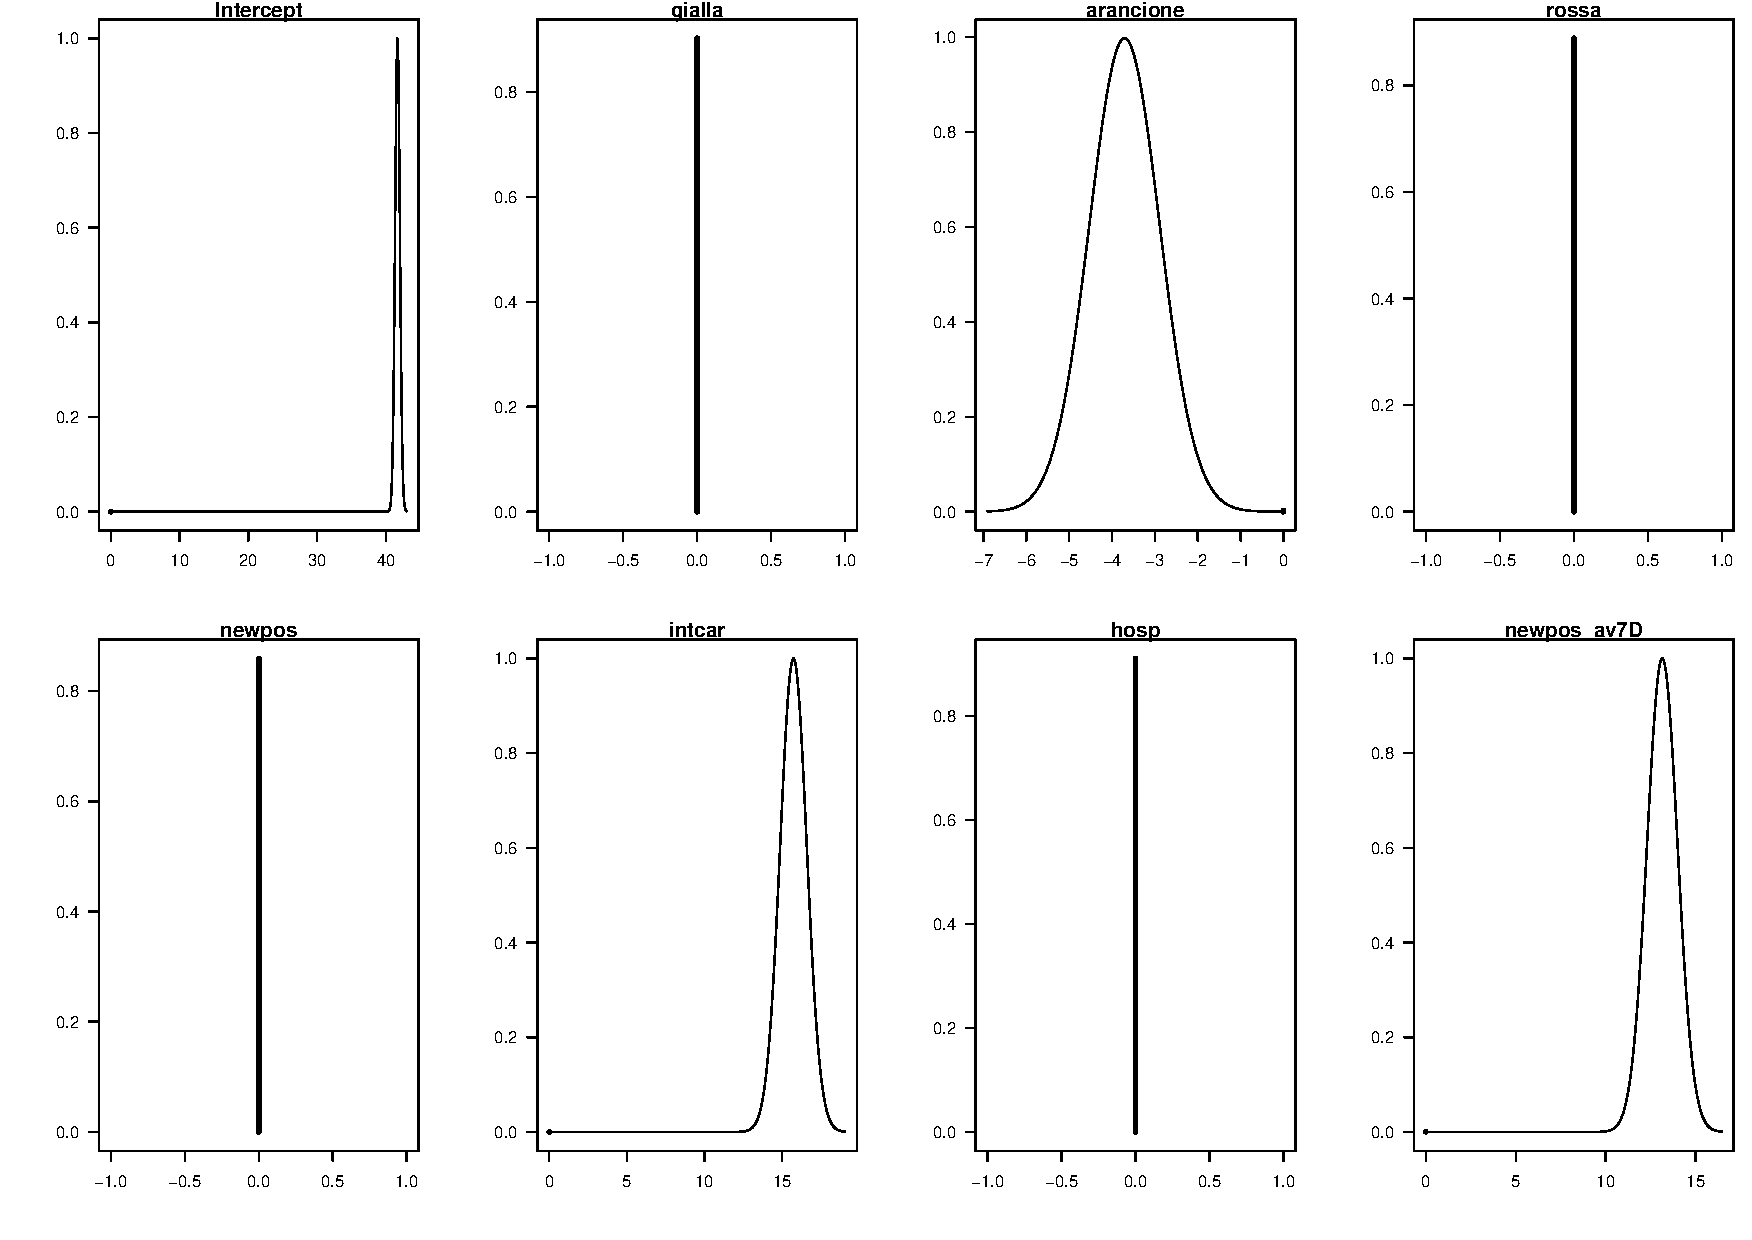
\includegraphics[width=140mm, height=90mm,scale=0.5]{posterior_2.pdf}
	\caption{Posterior distributions of coefficients for best \textbf{intcarH8} model}
\end{figure}

\begin{figure}[htb!]
	\centering
	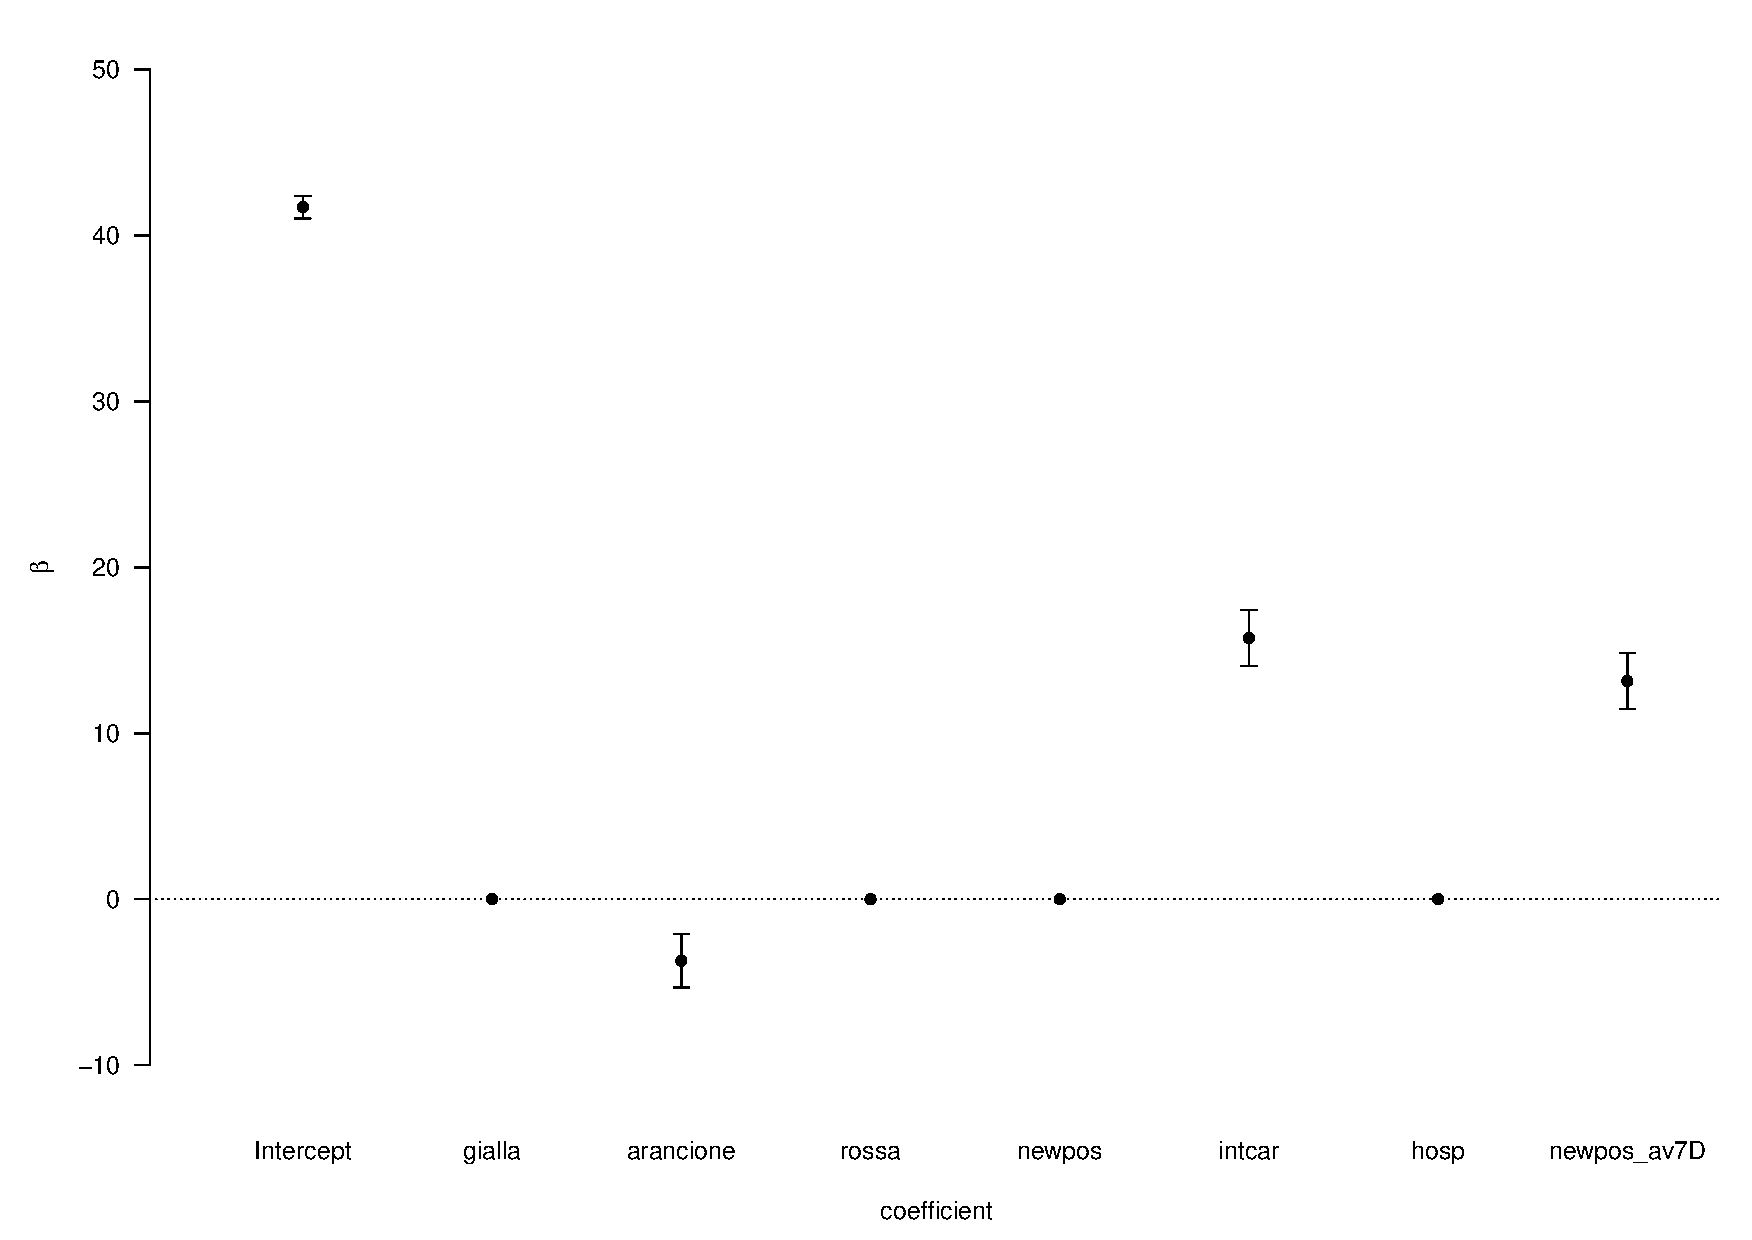
\includegraphics[width=140mm, height=90mm,scale=0.5]{crint2.pdf}
	\caption{95\% credible intervals for the coefficients in the \textbf{intcarH8} model}
\end{figure}

\clearpage
\newpage
\subsection{Sensitivity analysis}
Although we chose to be guided completely by the data,  we could still use a g-prior and tune the hyperparameter $\alpha$ by choosing the MSE as the criterion. We use the same models as before, so BMA with \textbf{hospH8} and the best model with 3 covariates for \textbf{intcarH8}.

In both cases the MSE is high for low values of $\alpha$. However, it decreases by increasing the value of $\alpha$ until it converges. We settle on $\alpha = 100$, as used in Subsection 2.1. 

Since there is no substantial difference in performance we kept using the non-informative prior with \texttt{BIC} in Subsections 2.3 and 3.1.

\section{Conclusion}
In conclusion we see that, given the evaluation based on MSE, the best models for predicting the target variables are the ones obtained via model selection using BIC. \\\\
An interesting thing to notice about these models is how different the covariates' inclusion probabilities are (see Table 1 and 2). In fact we see that for predicting the target \textbf{hospH8} the model cares whether the region is a red zone or not while for \textbf{intcarH8} the attention is shifted on the orange zone. This seems counterintuitive but if we take into account the fact the primary goal of the restrictions during the pandemic, here described by the color of the region, was to save hospitals from being overcrowded, it actually makes sense.
\clearpage
\begin{appendices}
	\section{Additional analysis}
	\subsection{Frequentist Linear Regression}
	In a frequentist setting we consider the following model 
	\begin{align*}
		y = \boldsymbol{\beta}^TX + \varepsilon
	\end{align*}
	where 
	\begin{align*}
		\varepsilon \sim \mathcal{N}(0, \sigma^2)
	\end{align*}
	We start by fitting the model selected in the Bayesian setting for \textbf{intcarH8}:
	\begin{dmath*}
		\textbf{intcarH8} = \beta_0 + \beta_1\textbf{arancione} +  \beta_2\textbf{intcar} + \beta_3\textbf{newpos\_av7D} + \varepsilon
	\end{dmath*}
	We fit the model with the training set and obtain an adjusted $R^2$ of 0.9462. We recall that $R^2$
	\begin{align*}
		R^2 = 1 - \frac{\sum_{i=1}^{n}(y_i-\hat{y_i})^2}{\sum_{i=1}^{n}(\overline{y}-\hat{y_i})}
	\end{align*}
	where $\overline{y}$ is the target mean in the training set, and $\hat{y_i}$  is our prediction of the $i$-th sample. Adjusted $R^2$ simply accounts for the degrees of freedom (number of covariates).  Figure 12 shows the diagnostics plots for the model. As we can see the residuals are clearly not Gaussian, and as a matter of fact a Shapiro test for normality returns a p-value close to zero. The residuals v. fitted plot seems to be random enough, and it appears the model has captured the variability of the data well enough. The MSE on the test set is 36.36943.
	
	\begin{figure}[htb!]
		\centering
		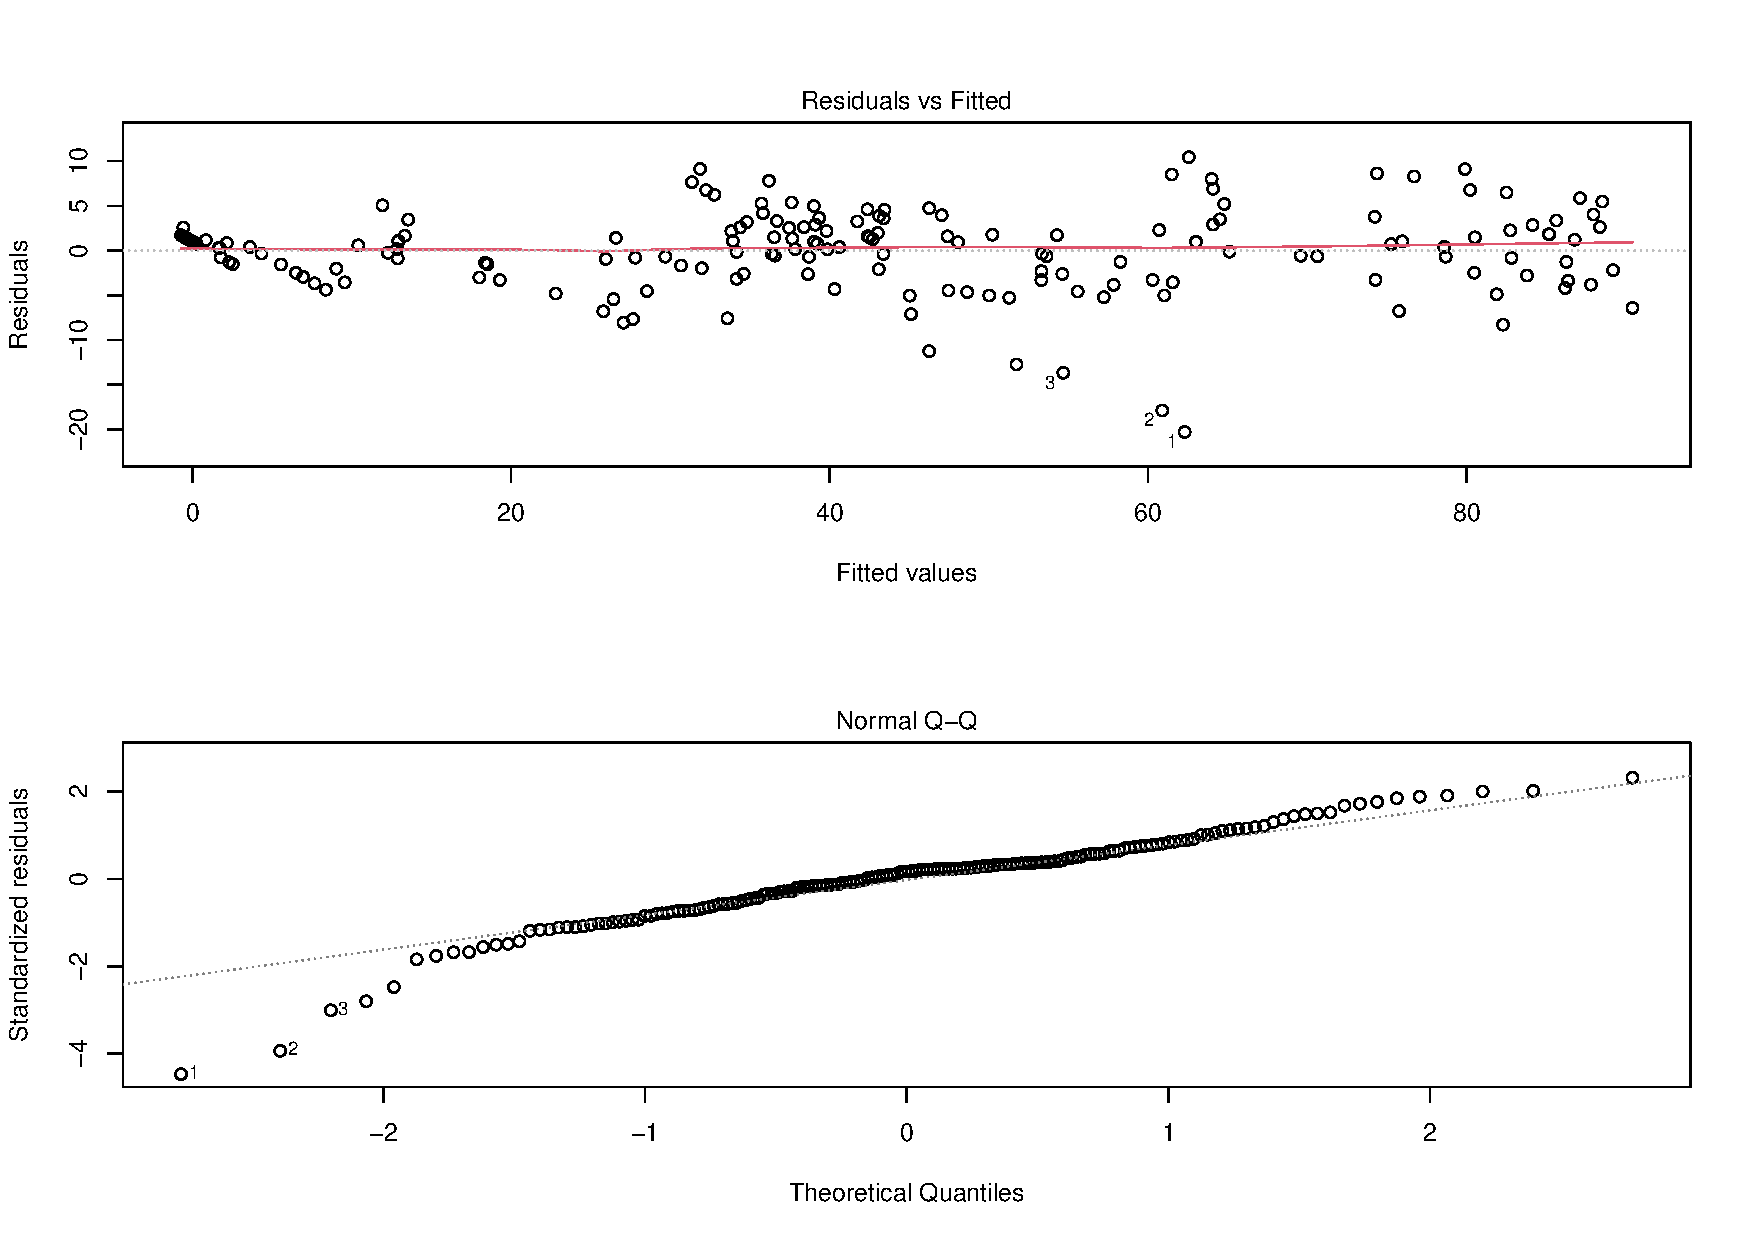
\includegraphics[width=100mm, height=90mm,scale=0.5]{diagnostics1.pdf}
		\caption{Diagnosis plots of the frequentist model for \textbf{intcarH8}}
	\end{figure}
	
	Lastly, we test the hypothesis $H_0: \,\,\, \beta_i = 0 \,\,\,\,\, v. \,\,\,\,\, H_1: \,\,\,\beta_i \neq 0$ for each coefficient. We reject each hypothesis at any significance level since all p-values are equal to zero, meaning that all the covariates contribute significantly to the model.
	
	For predicting \textbf{hospH8} we choose the best model found in the Bayesian case, to emulate the aggregate model we would have to resort to ensemble methods, which we avoid for simplicity. 
	
		\begin{dmath*}
		\textbf{hospH8} = \beta_0 + \beta_1\textbf{rossa} +  \beta_2\textbf{hosp} + \beta_3\textbf{newpos\_av7D} + \varepsilon
	\end{dmath*}
	
	We obtain an adjusted $R^2$ of 0.9836. Figure 13 shows the diagnostics plots for the model.  Again, the residuals do not pass a normality test, and we reject the null hypothesis for every covariate. We also do not see a complete random pattern in the residuals v. fitted plot, meaning there could be some complexity in the data that our model did not capture. The MSE on the test set is 752.7621.
	
		\begin{figure}[htb!]
		\centering
		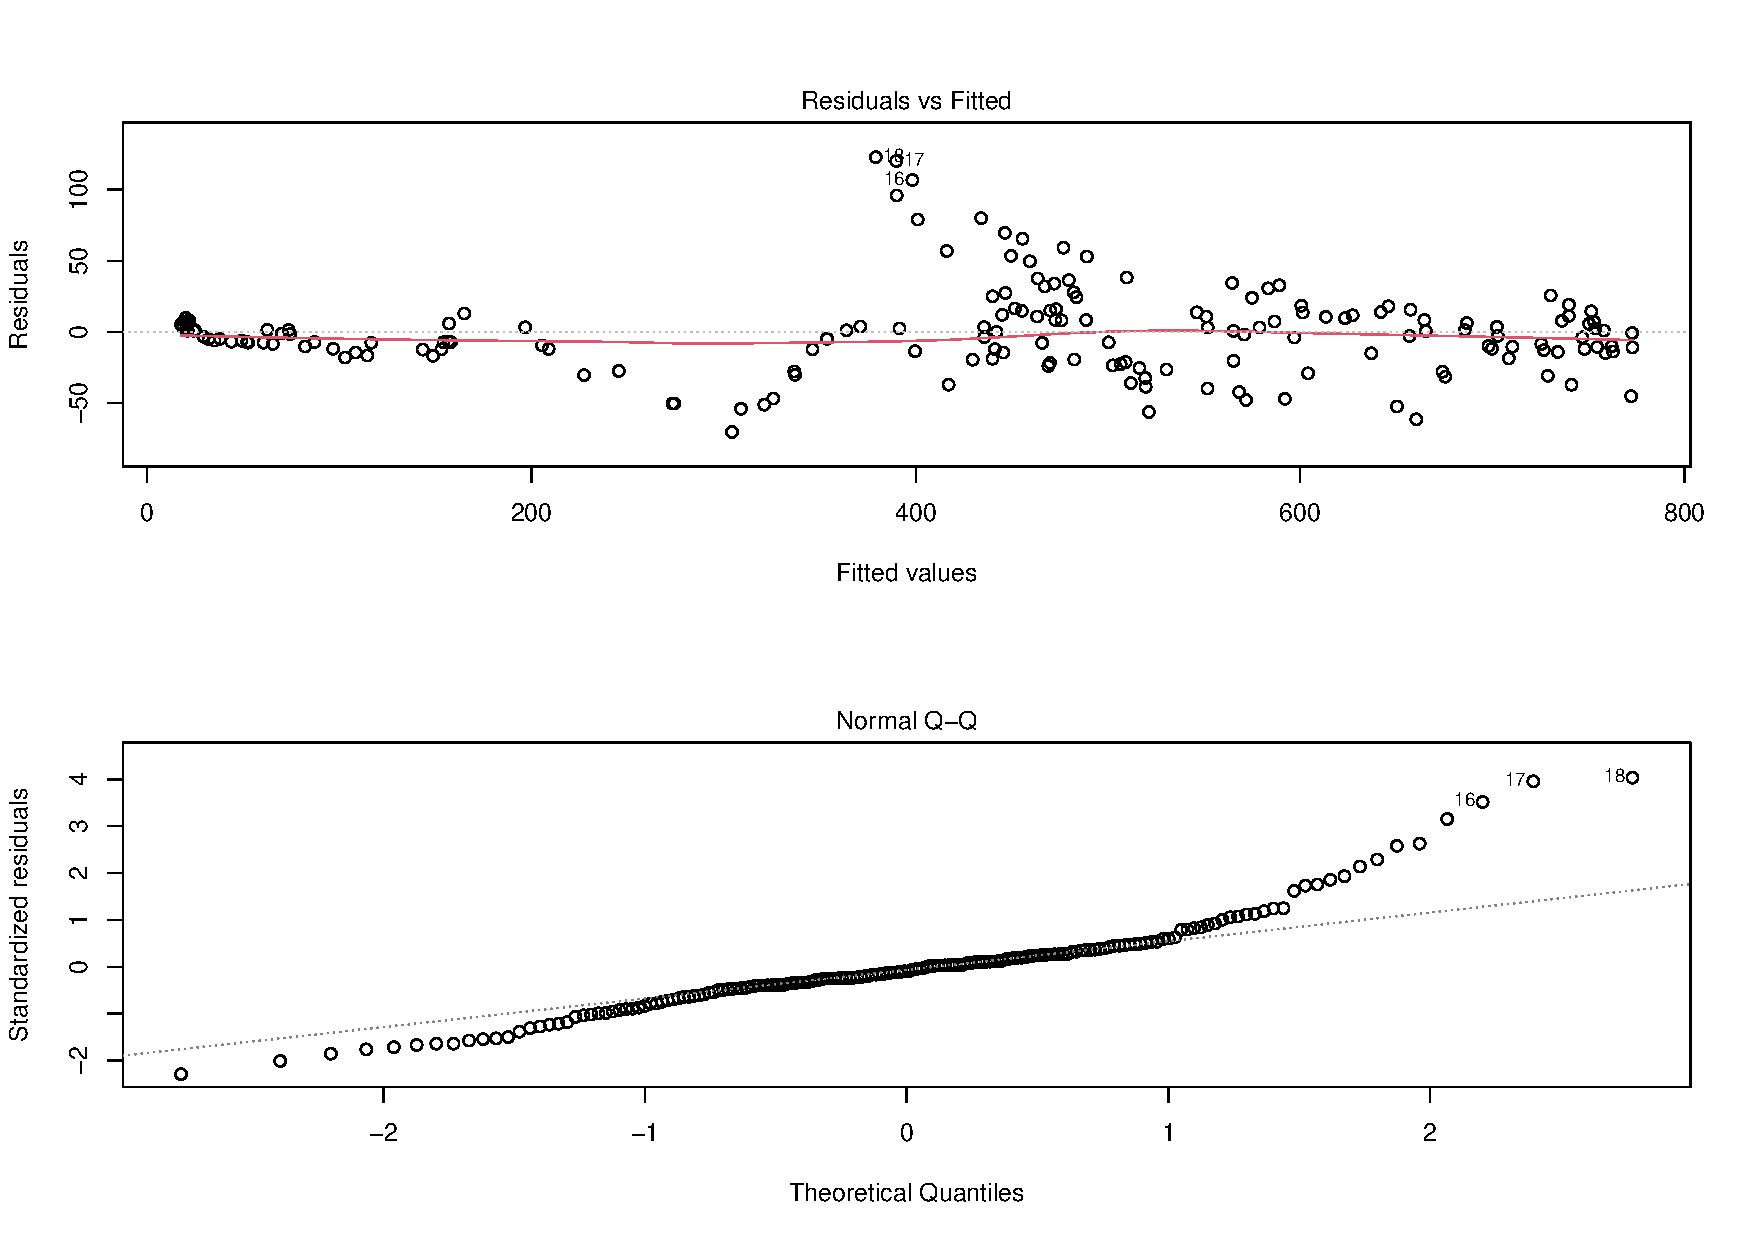
\includegraphics[width=100mm, height=90mm,scale=0.5]{diagnostics2.pdf}
		\caption{Diagnosis plots of the frequentist model for \textbf{hospH8}}
	\end{figure}

    \clearpage
    \subsection{Different representations of some covariates}
    \subsubsection*{Color as a numerical variable}
    This model considers the \textbf{color} covariate as an ordinal variable, note that this model uses the non-informative prior with BIC as the model selection criterion. The new covariate starts from 1 (\textit{Bianca}) and ends in 4 (\textit{Rossa}).\\
    
    For \textbf{intcarH8} the model becomes:
\begin{dmath*}
	\textbf{intcarH8} = \beta_0 + \beta_1\textbf{color}  + \beta_2\textbf{newpos} + \beta_3\textbf{intcar} + \beta_4\textbf{hosp} + \beta_5\textbf{newpos\_av7D} + \varepsilon
\end{dmath*}
which yields a MSE of 25.85215, slightly worse than the error of the other models. The same goes for \textbf{hospH8}, which yields a MSE of 1019.115, so we decide to drop this variant of our model.

\subsubsection*{Season}

Here we transform the variable \textbf{day} into \textbf{season} and include it in the model.

\begin{figure}[htb!]
	\centering
	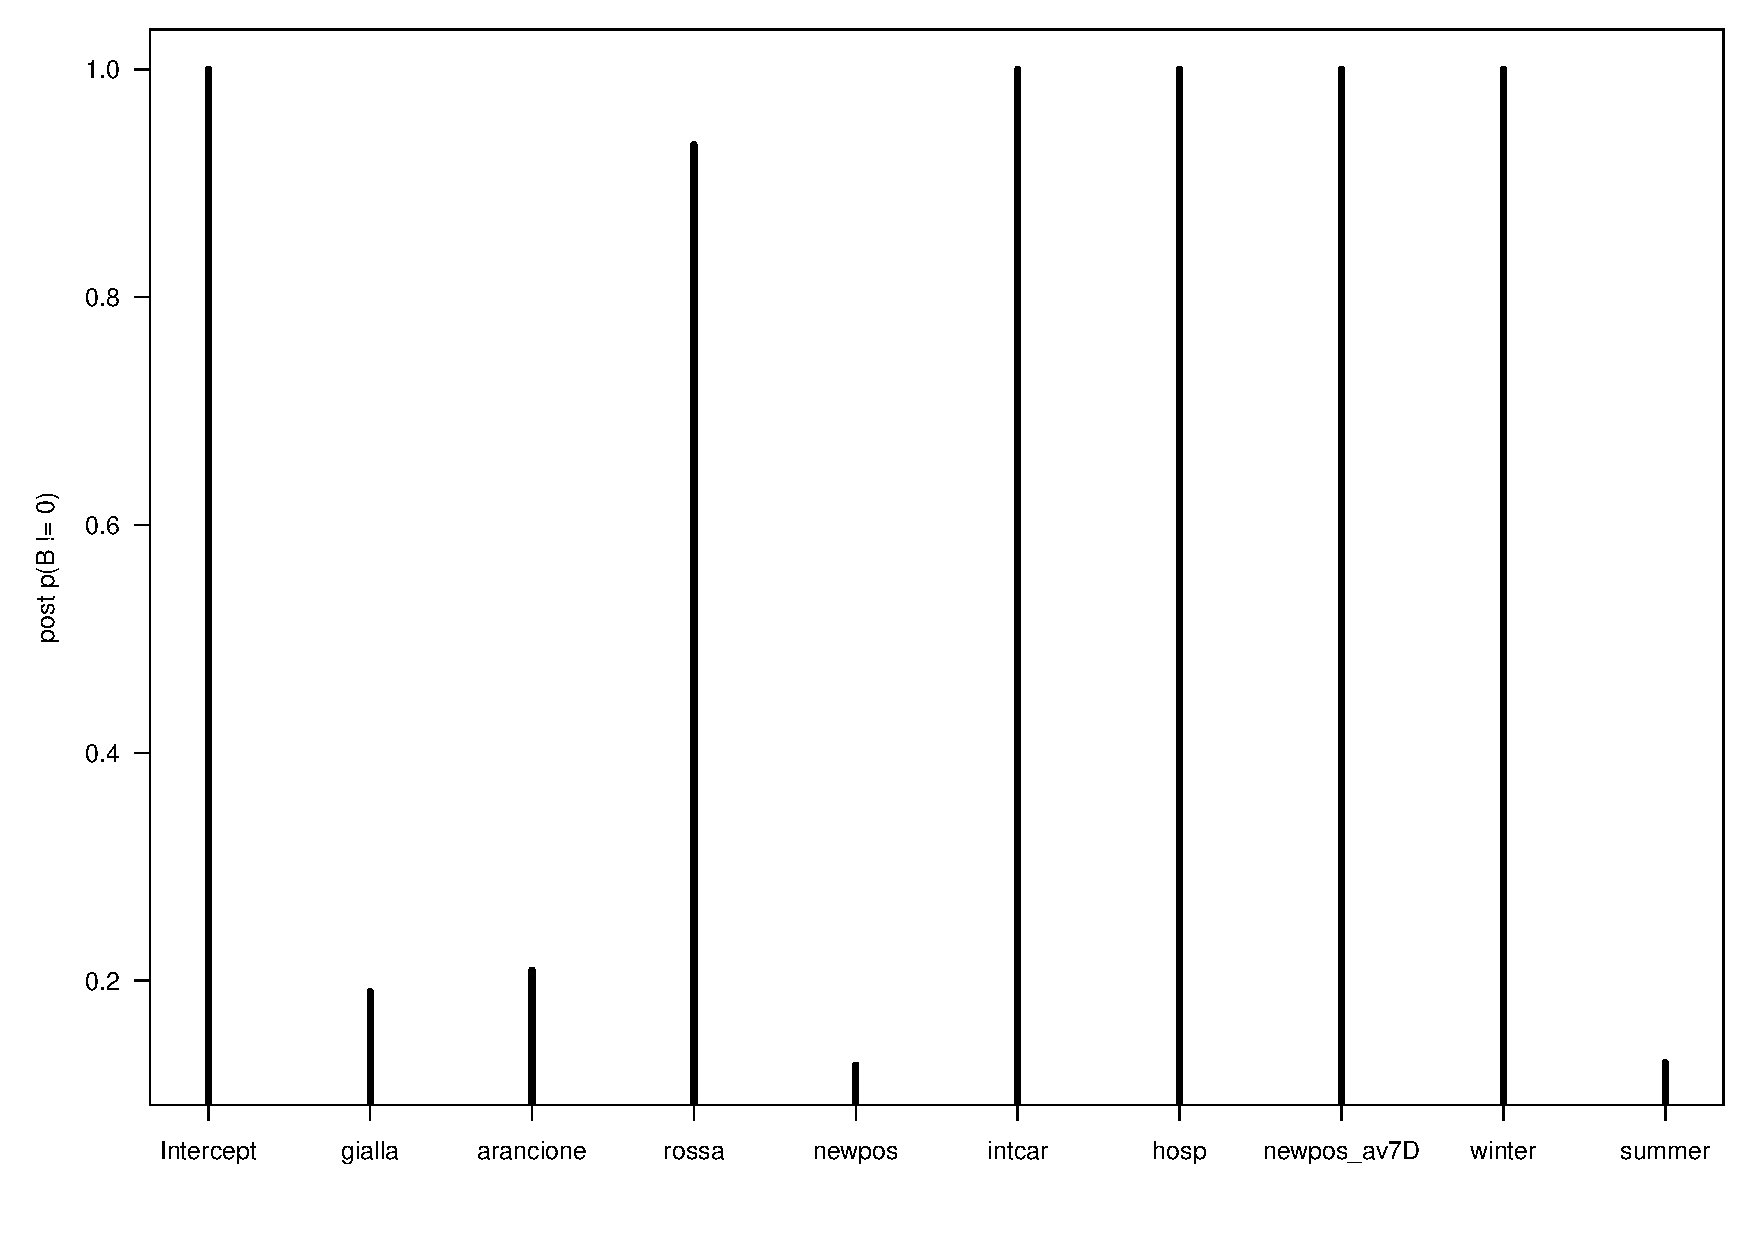
\includegraphics[width=140mm, height=90mm,scale=0.5]{szn1.pdf}
	\caption{Feature inclusion probabilities for \textbf{hospH8}.}
\end{figure}

As we can see in Figure 14, the \textbf{winter} indicator variable for the season (with target \textbf{hospH8}) seems to be relevant. Indeed the MSE of this model is 781.8348, which is the best one we achieved.

\begin{figure}[htb!]
	\centering
	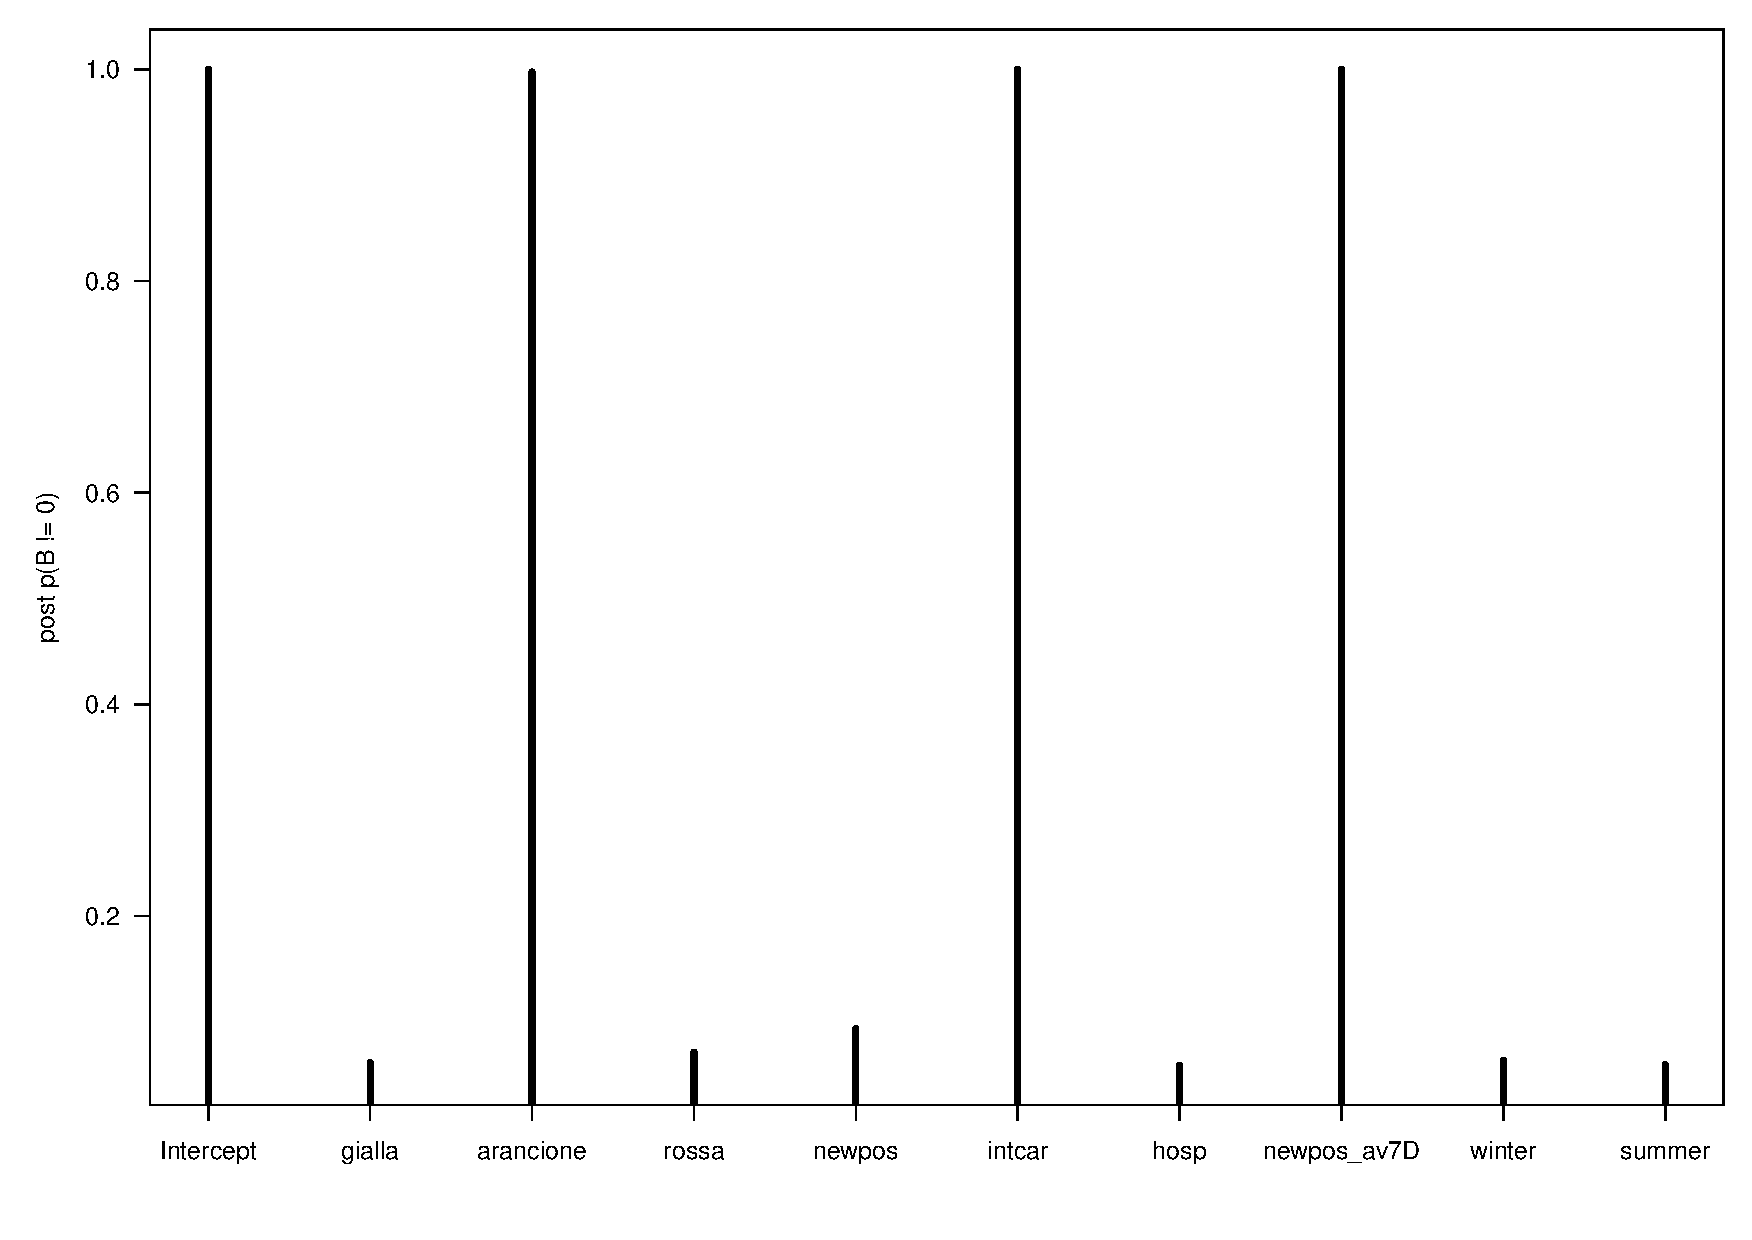
\includegraphics[width=140mm, height=90mm,scale=0.5]{szn2.pdf}
	\caption{Feature inclusion probabilities for \textbf{intcarH8}.}
\end{figure}

Instead in Figure 15 we can see that for the prediction of \textbf{intcarH8} the season doesn't seem relevant. Indeed the MSE results 23.0993, which is barely better than the other models without the season.
    
\end{appendices}
\end{document}